\documentclass[11pt]{article}
\usepackage[utf8]{inputenc}
\usepackage[T1]{fontenc}
\usepackage{lmodern}
\usepackage[margin=1in]{geometry}
\usepackage{graphicx}
\usepackage{amsmath}
\usepackage{amssymb}
\usepackage{booktabs}
\usepackage{longtable}
\usepackage{enumitem}
\usepackage{tcolorbox}
\usepackage{titlesec}
\usepackage{placeins}
\usepackage[round,authoryear]{natbib}
\usepackage[colorlinks=true,linkcolor=paperblue,citecolor=paperblue,urlcolor=paperblue,backref=page]{hyperref}
\tcbuselibrary{skins}

% Loosen float placement so tables/figures land near their reference
% instead of drifting to the end of the document.
\renewcommand{\topfraction}{0.9}
\renewcommand{\textfraction}{0.07}
\renewcommand{\floatpagefraction}{0.7}
\setcounter{topnumber}{4}
\setcounter{totalnumber}{6}

% ============================================================
%  Whitepaper: LaTeX source (sample-paper style)
%  Build with:  pdflatex main.tex && bibtex main && pdflatex main.tex && pdflatex main.tex
% ============================================================

\definecolor{paperblue}{RGB}{59,103,190}
\definecolor{titlebox}{RGB}{248,247,253}

\titleformat{\section}{\normalfont\sffamily\bfseries\large}{\thesection}{0.6em}{}
\titleformat{\subsection}{\normalfont\sffamily\bfseries}{\thesubsection}{0.6em}{}
\titlespacing*{\section}{0pt}{1.4em}{0.7em}
\titlespacing*{\subsection}{0pt}{1.1em}{0.5em}

\renewcommand{\bibsection}{\section*{References}}
\renewcommand*{\backref}[1]{}
\renewcommand*{\backrefalt}[4]{%
  \ifcase #1 (not cited)\or (page #2)\else (pages #2)\fi}

\setlength{\bibsep}{4pt}
\setlength{\emergencystretch}{2em}
\hypersetup{pdftitle={A Two-Layer Synthetic Data Generator for Studying Student Retention Early-Warning Systems in Philippine Higher Education},pdfauthor={Matthew C. Batitay},pdfsubject={Eskwelabs Innovation Fellowship, Data Innovation Track},pdfkeywords={synthetic data, student retention, early-warning systems, Philippine higher education, confounded intervention assignment}}

\begin{document}

\begin{tcolorbox}[colback=titlebox,colframe=titlebox,arc=4mm,boxrule=0pt,left=10mm,right=10mm,top=6mm,bottom=6mm]
\begin{center}
{\sffamily\bfseries\LARGE A Two-Layer Synthetic Data Generator for Studying Student Retention Early-Warning Systems in Philippine Higher Education}\\[10pt]
{\large Matthew C. Batitay}\\[2pt]
{\itshape Eskwelabs Innovation Fellowship, Data Innovation Track}
\end{center}
\vspace{6pt}

\noindent\textbf{Abstract.} Administrative records at Philippine higher-education institutions capture what a student does (grades, attendance, financial-account status) but rarely capture why a student leaves. Published figures on four-year cumulative attrition do not line up: a single CHED regional table reports two consecutive graduating cohorts whose regional rates differ by about nineteen percentage points on average, and the national figures in circulation, roughly three in ten and roughly four in ten students who begin a degree, do not appear to trace to the same cohort or source; Section~\ref{sec:calibration} traces them, states which cohort this model calibrates to, and states why. Whichever figure is used, the individual-level mechanisms behind these numbers are not present in any public dataset. This paper specifies a synthetic data model that reproduces this gap deliberately: a two-layer generative structure in which a latent state, meaning a student's structural vulnerability and exposure to acute shocks, drives both the observed institutional record and the eventual dropout outcome, while remaining itself unobservable to any downstream analyst. The model further encodes a confounded intervention-assignment mechanism, motivated by the documented tendency of early-warning systems to base support decisions on the same signals that predict the outcome, so that the effectiveness of a support program cannot be read off through naive comparison alone. Every generative parameter is tagged by provenance as locked, calibrated against cited Philippine statistics, or explicitly assumed, and the model's aggregate behavior is calibrated against national and regional attrition figures reported by the House of Representatives' Congressional Policy and Budget Research Department, the Second Congressional Commission on Education, and the Philippine Institute for Development Studies, and is checked against those figures via the calibration-loop procedure specified in Section~\ref{sec:validation}, a procedure that section distinguishes explicitly from a limited, pre-specified held-out check against a second graduating cohort. A pilot instantiation reported in Appendix~\ref{sec:appendixA} calibrates to the tier targets and reproduces the intended confounding, but shows that only estimators that borrow strength across signal cells recover the true effect, and its held-out check lands marginally outside the pre-specified band.
\end{tcolorbox}

\vspace{10pt}

\FloatBarrier
\section{Introduction}
\label{sec:intro}

National figures on Philippine higher education attrition describe a problem of substantial scale, though the figures themselves do not agree on its exact size. Reported four-year cumulative attrition sits somewhere between roughly three and four in ten students who begin a bachelor's degree, depending on which figure is used and which graduating cohort it describes (Section~\ref{sec:calibration} traces the figures to their cohorts and states which one this model calibrates to and why), and any national average conceals a wide regional spread: in CHED's own regional table, reported cumulative attrition for the Class of 2022 ranges from 36.3\% in the best-performing region to 93.4\% in the worst, and for the Class of 2023 from 8.0\% to 38.4\% (BARMM unreported) \citep{cpbrd2026}. These figures are collected and reported at the level of the region, the institution, or the cohort. They are not, and by design cannot be, collected at the level of the individual student whose specific circumstances led to a specific outcome.

This creates a structural gap between what an institution's information systems record and what actually determines a student's trajectory. A registrar's database holds grades, attendance flags, and the status of a tuition account. It does not hold, and generally has no lawful or practical way to hold, a reliable measure of a student's financial precarity, the stability of their household, or whether a single acute event, such as a medical emergency, a family crisis, or an unexpected expense, has just made continuing enrollment impossible. Qualitative research on Philippine dropout consistently identifies financial strain, family and employment pressures, and weak institutional support as dominant themes in students' own accounts of why they left \citep{cahilog2025,socioeconomic2024}, yet these same factors are almost never present as columns in an administrative dataset.

Because the individual-level data needed to study this gap does not exist publicly, and for reasons of privacy should not, any attempt to build or evaluate a retention early-warning system in this domain faces a basic evidentiary problem: the ground truth against which a model's predictions would ideally be checked is never observed, even by the institution generating the data. This paper addresses that problem from the opposite direction. Rather than attempting to obtain data that cannot ethically or practically be obtained, it specifies a synthetic data model that treats the gap between recorded and true state as the central object being modeled, rather than as noise to be engineered around.

The model described here separates every student's situation into two layers. An observed layer, consisting of grades, attendance, financial-hold status, and whether the student received institutional support, is generated so that it is exportable, analyzable, and structurally similar to what a real student-information system would contain. A latent layer, consisting of a fixed baseline vulnerability and a per-term probability of an acute shock, is generated to drive the observed layer and the eventual dropout outcome, but is never exported and is not visible to any analysis performed on the resulting dataset. That gap is deliberate: it is the mechanism by which the dataset reproduces the actual epistemic position of a Student Success Analyst (a title used with increasing frequency in Philippine and international higher-education administration for the staff role responsible for retention analytics and intervention targeting, though not yet a single standardized job title; it is used throughout this paper as a stand-in for whichever office at an institution owns that responsibility) working from institutional records alone.

The contribution of this paper is the data model itself: the entity structure, the latent-to-observed generative logic, the calibration targets drawn from published Philippine statistics, and the validation checks that any implementation of this model must satisfy. It does not present the generator's source code or the resulting dataset, which are separate deliverables built on the specification given here. The remainder of this paper is organized as follows. Section~\ref{sec:related} reviews the theoretical and empirical literature that motivates the model's structure. Section~\ref{sec:principles} states the design principles the model is held to. Section~\ref{sec:architecture} describes the entity inventory and end-to-end generation pipeline. Sections~\ref{sec:phase1}--\ref{sec:phase5} detail each of the pipeline's five phases. Section~\ref{sec:calibration} specifies the calibration parameters and their provenance tags. Section~\ref{sec:validation} defines the validation measures and success benchmarks. Section~\ref{sec:edgecases} describes two deliberately engineered edge cases. Section~\ref{sec:ethics} addresses ethical and responsible-use considerations specific to synthetic data of this kind. Section~\ref{sec:limitations} states the model's limitations and scope. Section~\ref{sec:conclusion} concludes. Appendix~\ref{sec:appendixA} gives a reference instantiation of the generative forms and reports a pilot check of the specification, and Appendix~\ref{sec:appendixB} gives the field-level schema and a reproducibility policy.


\FloatBarrier
\section{Related Work and Theoretical Foundation}
\label{sec:related}

\subsection{Classical Attrition Theory}
\label{sec:related-A}

Tinto's model of student departure frames dropout as the end point of insufficient academic and social integration into an institution, and remains the most widely cited theoretical account of college attrition \citep{tinto1975}. Bean and Metzner's later model extends this account for non-traditional students, arguing that external factors, including finances, employment, and family responsibility, dominate over campus-integration factors for students who are older, commuting, or working while enrolled \citep{bean1985}. Both models converge on the same structural claim that motivates this paper's design: the proximate, recordable events that precede a dropout (a missed class, a failed course, a lapsed payment) are downstream symptoms of a state that is not itself recorded anywhere. The two-layer generative structure in Section~\ref{sec:phase2} operationalizes this claim directly, rather than treating it as background motivation only.

\subsection{Machine-Learning Dropout Prediction and the Actionability Gap}
\label{sec:related-B}

A substantial and rapidly growing literature applies machine-learning classifiers to institutional and learning-management-system data to predict dropout, frequently reporting high predictive accuracy. A 2026 systematic review synthesizing 75 quality-assessed studies under PRISMA guidelines is explicit about what this literature has not yet established: despite strong predictive performance, there is limited evidence on how these models translate into empirically validated interventions in real institutional settings, a gap the review terms the actionability gap \citep{dropout2026review}. This distinction, between a model that predicts risk accurately and a program that demonstrably reduces it, is the reason this paper's data model treats prediction and intervention-effectiveness as two separate questions with two separate, independently checkable answers, rather than assuming that solving the first solves the second.

\subsection{Confounded Treatment Assignment in Educational Interventions}
\label{sec:related-C}

The actionability gap identified above has a specific statistical cause when institutions target support at already-identified at-risk students, which is the standard and sensible practice. Smith and Chimedza demonstrate through simulation that when treatment assignment depends on the same variables that predict the outcome, a naive comparison between treated and untreated groups yields a biased estimate of the treatment's true effect, and, critically for the design of any synthetic benchmark, that the size and direction of this bias can only be verified in a setting where the true effect is known by construction \citep{smith2021}. This paper adopts that same logic directly: Section~\ref{sec:phase4} specifies an intervention-assignment mechanism that is deliberately confounded by prior-term observed risk, and Section~\ref{sec:phase5} fixes a true intervention effect as an internal design constant, so that any downstream causal analysis performed on the resulting dataset has a known correct answer to be checked against.

\subsection{The Philippine Empirical Landscape}
\label{sec:related-D}

Three government and quasi-government sources anchor this model's calibration targets, and this paper is explicit about which specific figures come from which report rather than treating ``EDCOM~II'' as a single undifferentiated citation. The House of Representatives' Congressional Policy and Budget Research Department reproduces CHED's own regional attrition figures for two consecutive graduating cohorts, alongside enrollment and institution counts per region, in its FY2026 Agency Budget Notes for CHED \citep{cpbrd2026}. The Second Congressional Commission on Education's Year One report (2024) reports, among other findings, on the targeting of tertiary subsidies, and is not the source of the attrition figures used here; its Year Two report (2025) is the actual source of the specific national and regional figures ($\approx$39\% nationally, and figures for BARMM, Region VII, Region IX, and CAR individually) that CPBRD's own FY2026 Agency Budget Notes later reproduce, in its own narrative account of a legislator's floor speech, rather than as CPBRD's own computed statistic \citep{edcom2024,edcom2025y2}. This provenance chain, traced directly rather than assumed, is central to the resolution of the national-attrition discrepancy in Section~\ref{sec:calibration} and is the reason this paper does not treat the EDCOM II figure and the CPBRD-quoted figure as two independent corroborating sources. The Philippine Institute for Development Studies independently confirms the pandemic-era rise in national attrition and situates it within broader concerns about CHED's regulatory and developmental capacity \citep{pids2024}. Qualitative work at the institutional level, including a 2025 phenomenological study of dropped-out students at a tuition-free public HEI, identifies financial struggles, family obligations, low academic readiness, and weak institutional support as drivers of dropout \citep{cahilog2025}, with similar socioeconomic correlates reported in state-university-level research \citep{socioeconomic2024}. Together these sources establish both the aggregate scale of the phenomenon and its qualitative drivers, without ever providing, because no source of this kind could, the individual-level record that would let a researcher observe both the hidden state and the recorded state for the same student at the same time.


\FloatBarrier
\section{Design Principles}
\label{sec:principles}

Five principles govern every modeling decision made in the sections that follow. They are stated here so that any specific choice in Sections~\ref{sec:phase1}--\ref{sec:edgecases} can be checked against a stated intention rather than accepted on its own authority.

\begin{itemize}[topsep=2pt,itemsep=3pt,parsep=0pt]
\item \textbf{Empirical Fidelity:} every aggregate quantity the generator produces that has a real published counterpart (a national attrition rate, a regional split, a driver's relative prevalence) must reproduce that counterpart within a stated tolerance of ±3 percentage points (Section~\ref{sec:validation}), and the source of that counterpart must be citable. Two quantities are handled differently, and Sections~\ref{sec:calibration} and~\ref{sec:validation} say how: the pooled national rate is derived from the tier targets and is not matched to a national headline figure, and the held-out tier ratio has its own pre-specified band.
\item \textbf{Deliberate Opacity:} the gap between what is recorded and what is true reflects a deliberate modeling choice rather than an incomplete one: it is modeled directly, so that a downstream analyst working only from the exported tables faces the same informational limits a real Student Success Analyst (Section~\ref{sec:intro}) would face.
\item \textbf{Full Traceability:} every parameter that enters the generator is tagged as fixed by design, calibrated against a cited source, or explicitly assumed, and no parameter is permitted to carry an unstated status.
\item \textbf{Built-In Falsifiability:} the model fixes at least one quantity, the true effect of the support intervention, that is unknowable in any real dataset but known here by construction, so that a downstream causal analysis has a correct answer to be scored against rather than only a plausible-looking one.
\item \textbf{Bounded Scope:} granularity is capped at the level the cited real statistics can actually support; where a real number exists only at the national or two-tier regional level, the model does not manufacture false precision by fitting seventeen individual regions to it.
\end{itemize}


\FloatBarrier
\section{System Architecture and End-to-End Pipeline}
\label{sec:architecture}

Six of the model's eight tables use a panel structure, one row per student per academic term, rather than a single record per student; the remaining two (Regions and Students) are fixed at generation time. This is a substantive structural choice, not a formatting convenience. A question of the form ``will this student leave next term'' is a question about a sequence of states, and answering it, whether inside the model or in any downstream analysis of the resulting data, requires the sequence to be present in the data as a sequence. In the statistical literature this is referred to as a person-period or discrete-time panel, the standard representation for discrete-time survival analysis, in which a term is the unit of time and a dropout is either an observed event or a right-censored non-event for students still enrolled at the end of the observation window.

Generation proceeds through five phases, shown in Fig.~\ref{fig:pipeline}. Phases 1--4 and the per-term draw in Phase 5 (labeled Phase 5a in Fig.~\ref{fig:pipeline}) run in a fixed order for each synthetic student's full enrollment history. Phase 5's aggregate check against real benchmarks (labeled Phase 5b) is a distinct, batch-level operation: it can only run once the entire cohort of $N$ students has been generated, not per student, and its output is used to recalibrate the numeric parameters set in Phases 1 and 2 before the generator is considered final; this is the dashed feedback path in Fig.~\ref{fig:pipeline}. This closed loop of parameter setting, output generation, and output analysis against real benchmarks follows standard input-modeling and verification-and-validation practice for discrete-event and Monte Carlo simulation models, in which a model is not accepted as final until its generated output has been checked against real-world reference data \citep{law2015}; Section~\ref{sec:validation} states explicitly why this closed loop, because it tunes parameters against the same benchmarks it is then checked against, should be read as calibration-until-convergence rather than as independent held-out validation.

\begin{figure}[t]
\centering
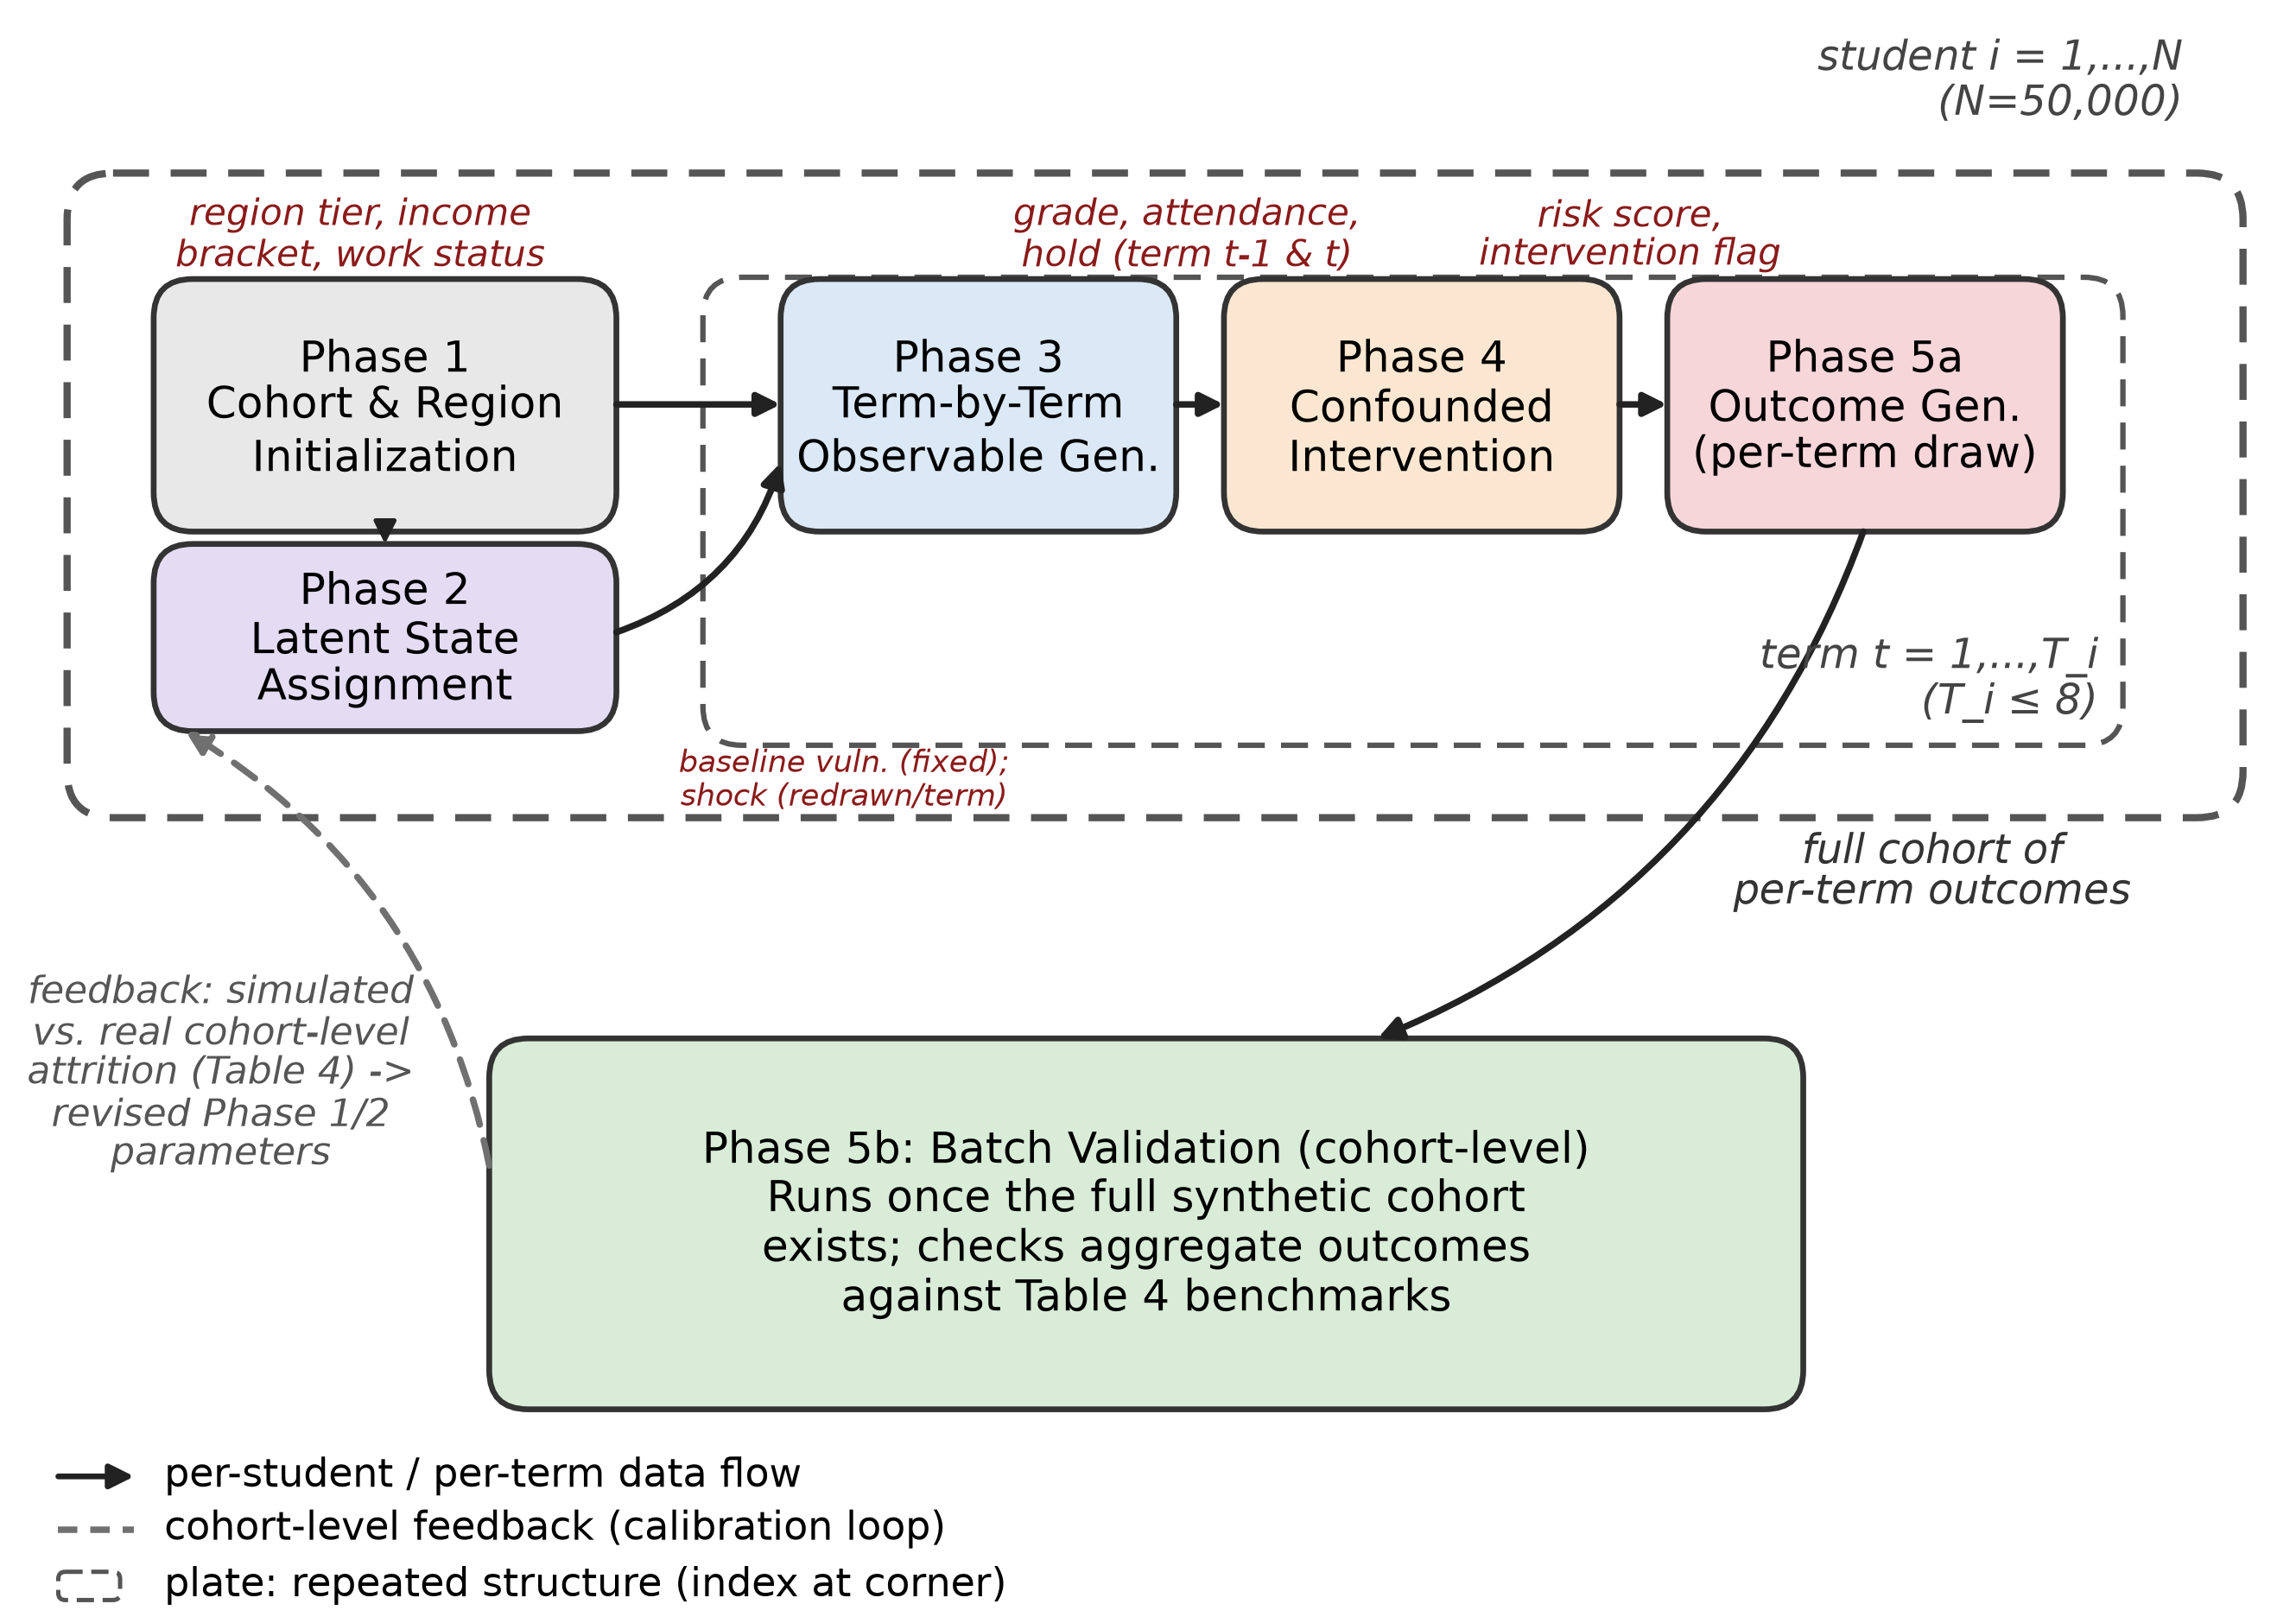
\includegraphics[width=6.3in]{figures/fig1_pipeline.png}
\caption{End-to-end synthetic cohort generation pipeline. The outer plate (student $i=1,\ldots,N$, $N=50{,}000$) and inner plate (term $t=1,\ldots,T_i$, $T_i \le 8$) show the two levels of repetition described in Section~\ref{sec:architecture}. Phases 1--4 and the per-term outcome draw (5a) repeat inside these plates; batch validation (5b) is drawn outside both plates because it is a cohort-level operation that runs once, after the full synthetic cohort exists, not a per-student or per-term step. The dashed arrow is the calibration feedback path, not a data-generation step.}
\label{fig:pipeline}
\end{figure}

\begin{table}[htbp]
\caption{Generation pipeline phases}
\label{tab:phases}
\centering
\small
\renewcommand{\arraystretch}{1.2}
\begin{tabular}{@{}p{0.24\textwidth}p{0.68\textwidth}@{}}
\toprule
\textbf{Phase} & \textbf{Activity} \\
\midrule
Phase 1: Cohort and Region Initialization & Each synthetic student is assigned a region tier, entry year, program discipline, income bracket, working-student status, and other fixed entry attributes. These are the only quantities generated before any latent state exists. \\
\addlinespace
Phase 2: Latent State Assignment & A fixed baseline vulnerability is drawn as a function of the Phase 1 attributes. A per-term shock indicator is set up to be drawn independently in every subsequent term. Neither quantity is exported. \\
\addlinespace
Phase 3: Term-by-Term Observable Generation & For each term in sequence, term grade, attendance rate, and financial-hold status are drawn as noisy functions of the current baseline vulnerability and that term's shock draw. \\
\addlinespace
Phase 4: Confounded Intervention Assignment & From a student's second term onward, an observed risk score is computed from the prior term's grade, attendance, and financial-hold values only. Whether the student receives a support intervention this term is drawn as a Bernoulli trial with that score as its probability (Eq.~\ref{eq:risk}--\ref{eq:intervention}); no intervention is assigned in term 1, which has no prior term (Section~\ref{sec:phase4}). \\
\addlinespace
Phase 5a: Outcome Generation (per student-term) & Whether the student drops out this term is drawn as a Bernoulli trial (Eq.~\ref{eq:hazard}--\ref{eq:dropout}) whose probability is the dropout hazard defined in Eq.~\ref{eq:hazard}, itself a function of baseline vulnerability, the current shock, and whether the student received a support intervention this term. \\
\addlinespace
Phase 5b: Batch Validation (per cohort, once) & After the full synthetic cohort of $N$ students has been generated, aggregate outcomes are checked against the real benchmarks in Table~\ref{tab:validation} before the parameters are finalized; see the calibration-loop discussion in Section~\ref{sec:validation}. \\
\bottomrule
\end{tabular}
\end{table}

Eight tables hold the model's output, listed in Table~\ref{tab:entities}. Six carry the student-term grain described above; the remaining two, Regions and Students, are fixed at generation time and do not repeat per term.

\begin{table}[htbp]
\caption{Entity inventory}
\label{tab:entities}
\centering
\small
\renewcommand{\arraystretch}{1.2}
\begin{tabular}{@{}p{0.20\textwidth}p{0.16\textwidth}p{0.55\textwidth}@{}}
\toprule
\textbf{Table} & \textbf{Grain} & \textbf{Contents} \\
\midrule
Regions & one per tier & Reference values used to calibrate regional attrition targets (Section~\ref{sec:calibration}). \\
\addlinespace
Students & one per student & Fixed entry attributes: region, entry year, program, income bracket, working-student status, distance from campus, subsidy status, and the latent baseline vulnerability (not exported). \\
\addlinespace
Enrollments & student $\times$ term & Enrollment status and the end-of-window censoring flag. \\
\addlinespace
CourseGrades & student $\times$ term & Term average score (0--100 scale), units attempted and passed. \\
\addlinespace
AttendanceRecords & student $\times$ term & Attendance rate for the term. \\
\addlinespace
FinancialHolds & student $\times$ term & Financial-hold status, overdue amount, and subsidy status for the term. \\
\addlinespace
SupportInterventions & student $\times$ term & The observed risk score (undefined in a student's first term) and whether an intervention was received (a single undifferentiated flag, always 0 in term 1; Section~\ref{sec:limitations} states why no intervention-type field is included). \\
\addlinespace
PersistenceOutcomes & student $\times$ term & The dropout flag for the term and the rolled-up cohort attrition flag used for validation. \\
\bottomrule
\end{tabular}
\end{table}

Sections~\ref{sec:phase1}--\ref{sec:edgecases} specify each table at the level of its grain, its role in the generative pipeline, and its provenance tags. The field-level column schemas and data types are given in Appendix~\ref{sec:appendixB}, and one admissible instantiation of the generative forms for the observed variables, used to check the specification in a pilot, is given in Appendix~\ref{sec:appendixA}; both are kept out of the main text so that the architectural argument is not obscured by implementation detail, and an implementation may differ from Appendix~\ref{sec:appendixA} provided it respects the constraints stated in Sections~\ref{sec:phase1}--\ref{sec:phase5}.

The generator is specified to produce a synthetic cohort of 50,000 students [LOCKED, a scale decision rather than a calibrated one], each followed for up to eight terms. This size is chosen so that the tier-level validation check in Section~\ref{sec:validation} is statistically meaningful despite the high-attrition tier holding only about 15\% of the population (Section~\ref{sec:calibration}): at that share, the tier still contains roughly 7,500 students, and a back-of-envelope binomial calculation puts the sampling error of a simulated attrition rate near 67\% at that sample size on the order of half a percentage point ($\sqrt{0.67 \times 0.33 / 7{,}500} \approx 0.0054$, i.e. $\approx$0.5 pp). This number should be read as an order-of-magnitude sanity check, not a precise error bound: the 15\% tier-share figure feeding into it, while shown against CPBRD's own enrollment data to sit within a citable plausible range (Table~\ref{tab:params}), is itself only pinned down to 14.1--18\% by that source, not fixed by it, so reporting a downstream sampling-error calculation to two decimal places would still overstate its precision. The substantive conclusion it supports is more modest and more robust to that imprecision: sampling noise at $N=50{,}000$ is comfortably an order of magnitude smaller than the $\pm$3-percentage-point tolerance in Section~\ref{sec:validation} across that entire plausible tier-share range, so a validation failure at that threshold would reflect a genuine miscalibration rather than ordinary sampling noise.


\section{Phase 1: Cohort and Region Initialization}
\label{sec:phase1}

Every synthetic student begins with a fixed set of attributes drawn independently of any later state: a region tier, an entry year, a program discipline, a household income bracket, working-student status, distance from campus, and subsidy status at entry. Region tier is the single most consequential of these attributes, because it is the attribute through which the model connects to the largest and most reliable real benchmark available: published regional attrition figures.

Reported four-year cumulative attrition varies widely across Philippine regions within each graduating cohort: CPBRD's regional table reports 36.3\% to 93.4\% across regions for the Class of 2022 and 8.0\% to 38.4\% for the Class of 2023 (BARMM unreported), and it falls by about 19 percentage points on average per region from the first of these cohorts to the second \citep{cpbrd2026}. Modeling all regions individually would require region-specific calibration data this project does not have at sufficient granularity, and would produce an appearance of precision the underlying sources cannot support. The model instead groups regions into two tiers. The high-attrition tier is composed of the four regions with the highest reported cumulative attrition in CPBRD's regional table \citep{cpbrd2026}, specifically its Class-of-2022-cohort column: BARMM at 93.4\%, Region VII at 60.7\%, Region IX at 59.5\%, and CAR at 54.9\%, all well above the 36.3\% figure (Region II) at the low end of the same column. (The Region IX figure is the one CPBRD's own infographic table reports; the same CPBRD document's narrative text separately states 59.9\% for Region IX when reporting a legislator's floor speech -- a source-internal inconsistency this paper did not create and resolves by using the tabulated figure throughout, as discussed further in Section~\ref{sec:calibration}.) These four figures are also independently reproduced exactly in EDCOM~II's Year Two report \citep{edcom2025y2}; the 59.9\% figure is unique to CPBRD's own narrative account of the floor speech and does not appear in EDCOM~II's report at all, which if anything strengthens confidence in the tabulated regional figures even though, as Section~\ref{sec:calibration} discusses, the same cannot be said for the national total. The typical tier comprises all remaining regions (thirteen, all with reported values). This two-tier grouping is a deliberately coarse stand-in for what a fully hierarchical model would instead treat as region-level random effects nested within a national distribution \citep{gelman2013bda}; it is a scope decision stated openly here and revisited as a limitation in Section~\ref{sec:limitations}, not a constraint discovered after the fact. Section~\ref{sec:calibration} gives the specific numeric targets attached to each tier.


\FloatBarrier
\section{Phase 2: Latent State Assignment}
\label{sec:phase2}

Two quantities generated in this phase are never exported to any table and are not accessible to any analysis performed on the resulting dataset. Their role is to be the true, unobserved cause of everything that follows.

Baseline vulnerability is a continuous value fixed once per student at entry, generated as a function of region tier, income bracket, and working-student status. It represents a student's structural exposure to the pressures identified in Section~\ref{sec:related} as the dominant drivers of Philippine attrition, namely financial precarity and competing employment demands, and is deliberately not observable in the same way those pressures are not directly recorded in any real student-information system.

Term shock is a per-term indicator, redrawn independently every term with probability $\pi_s$ (Table~\ref{tab:params}), representing an acute disruption uncorrelated with the student's baseline standing: a medical event, a family emergency, an unplanned expense. Its independence from baseline vulnerability is a specific and load-bearing design choice: it is what allows a student with a low baseline vulnerability and no adverse recorded history to still leave, which is the mechanism behind the first edge case in Section~\ref{sec:edgecases}. Fig.~\ref{fig:dag} shows the complete causal structure connecting these two latent quantities to every observed and derived quantity described in Sections~\ref{sec:phase3}--\ref{sec:phase5}, drawn in the probabilistic-graphical-model convention used throughout the Bayesian modeling literature to distinguish random variables from deterministic functions and observed quantities from latent ones \citep{mcelreath2020,gelman2013bda}.

\begin{figure}[htbp]
\centering
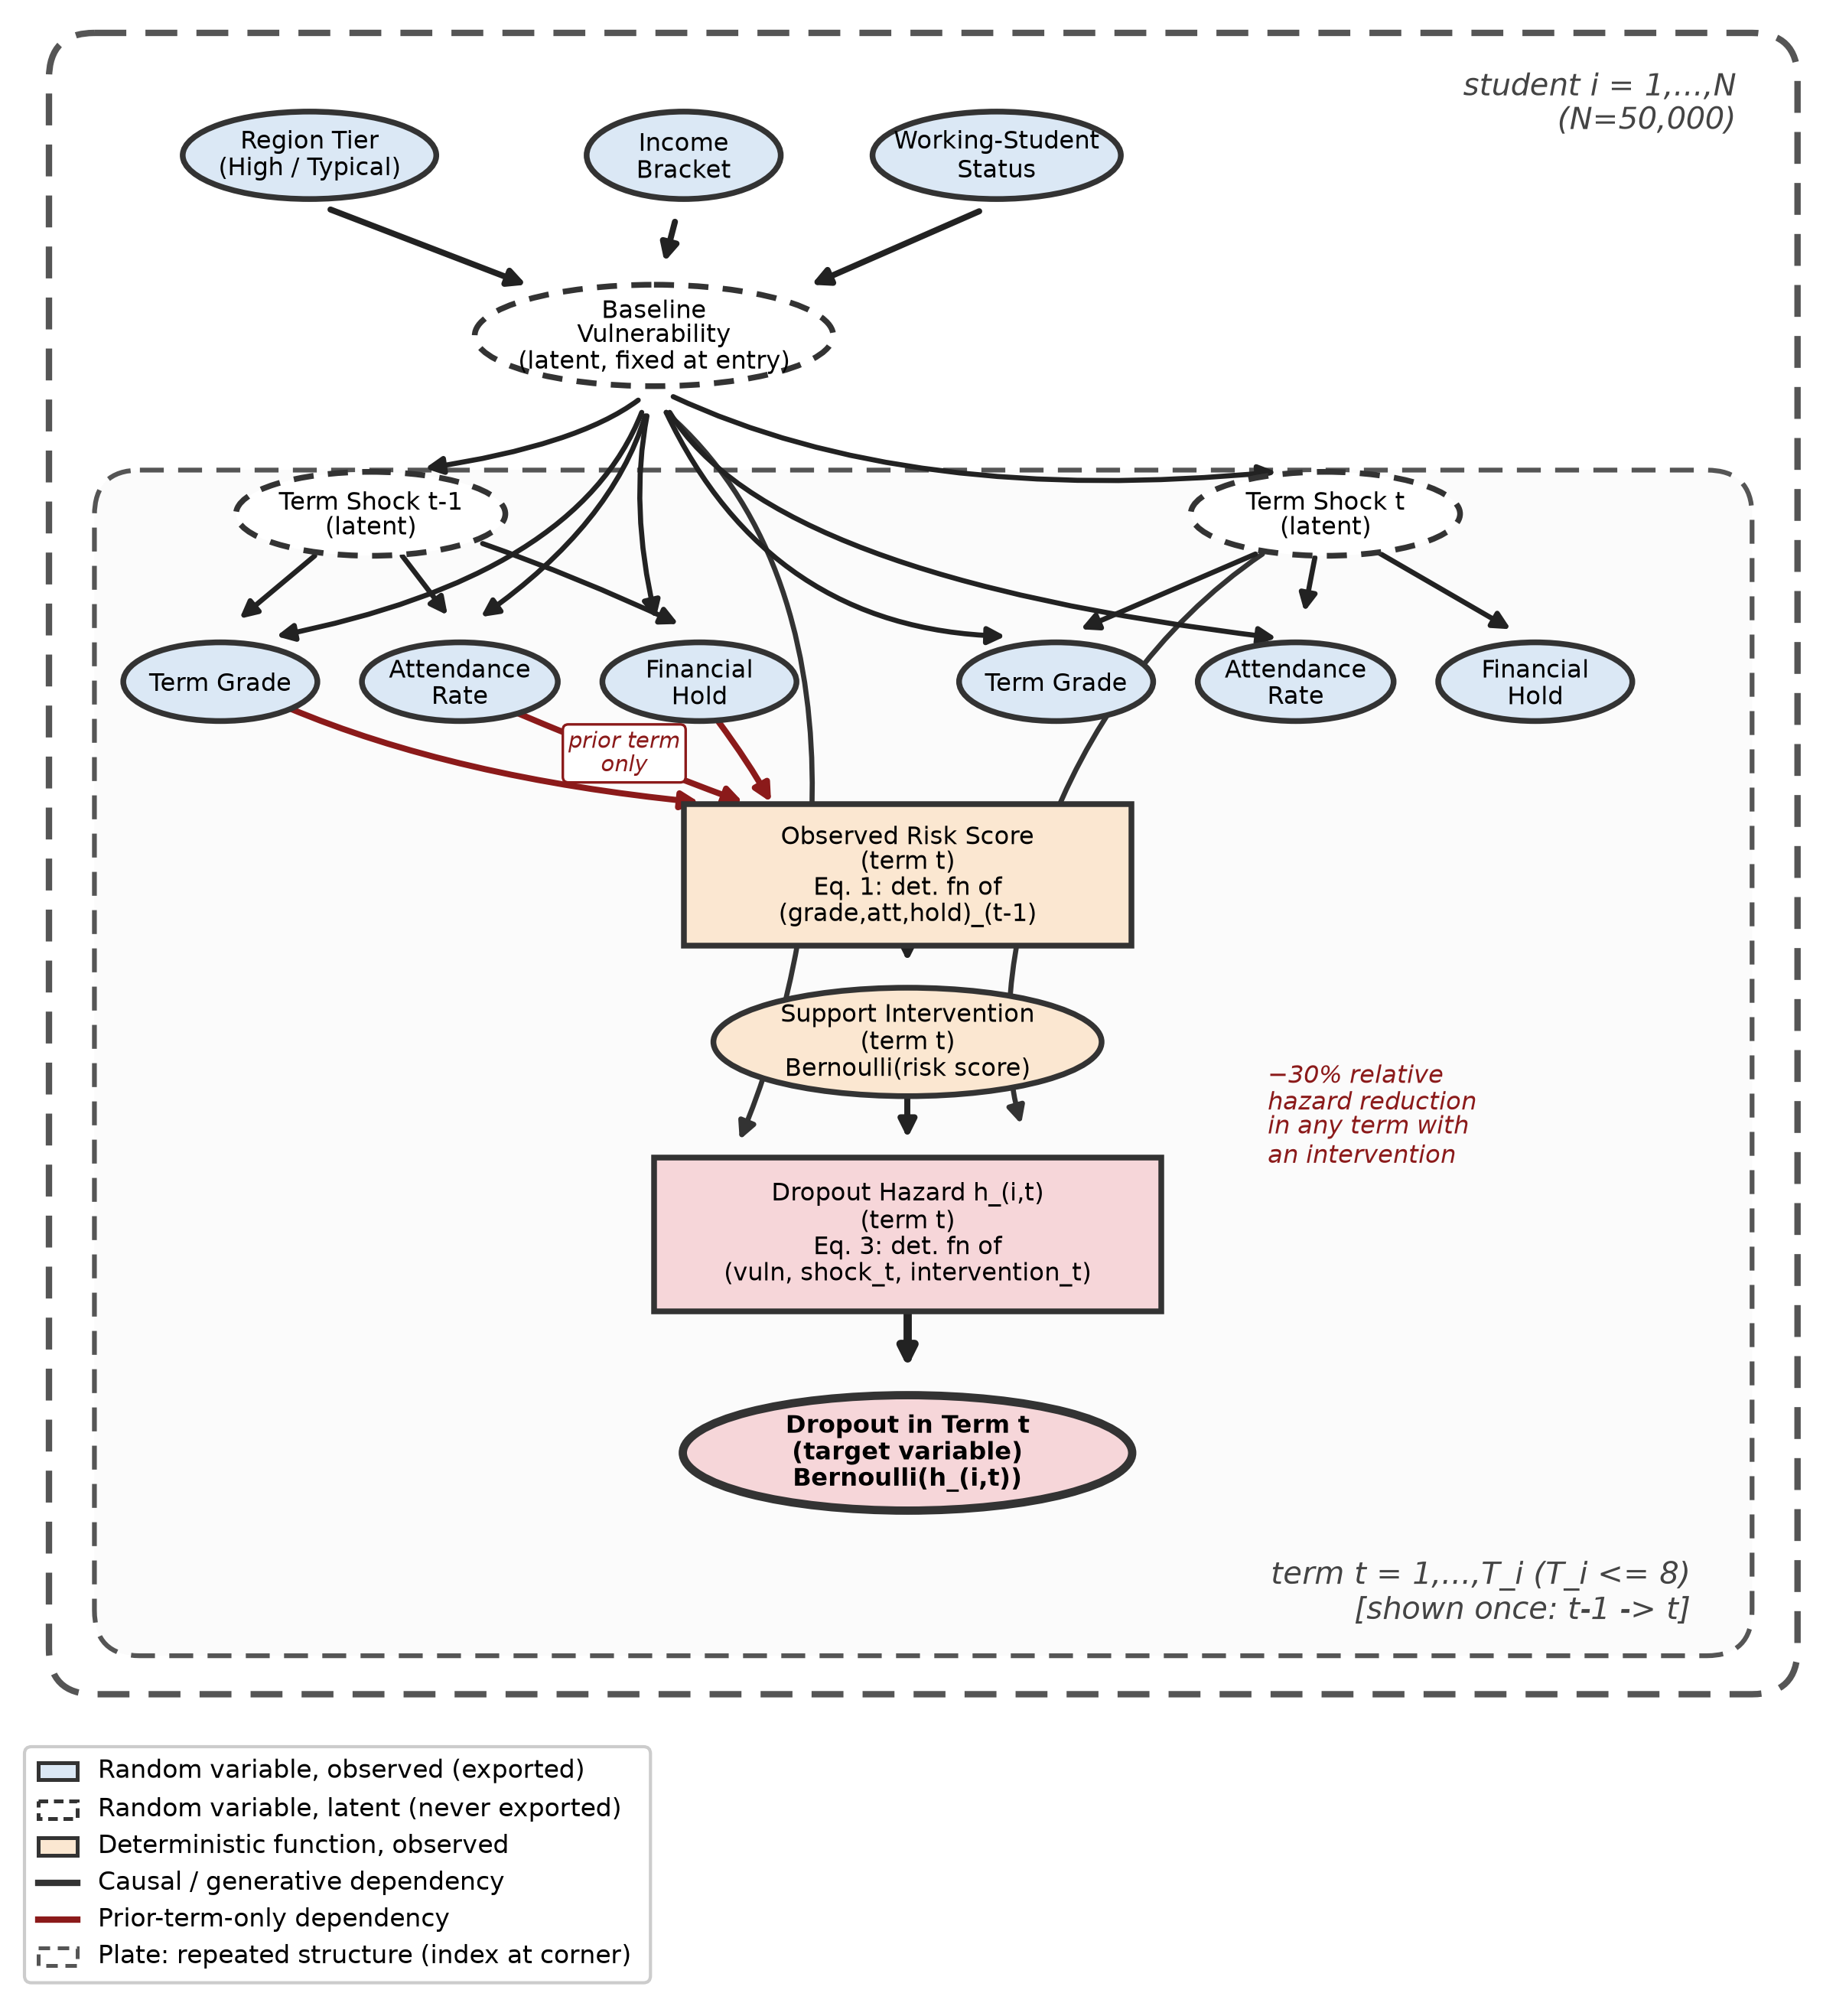
\includegraphics[width=5.6in]{figures/fig2_dag.png}
\caption{Latent and observed causal structure of the generative model. Following standard PGM convention, circles/ellipses denote random variables and rectangles denote deterministic functions of their parents; shaded (colored) nodes are exported to the dataset, and white nodes with dashed outlines are latent and never exported. The outer plate is the per-student repetition ($i=1,\ldots,N$); the inner plate is the per-term repetition ($t=1,\ldots,T_i$, $T_i \le 8$), shown unrolled once across an adjacent term pair $t-1 \to t$ to make the prior-term-only dependency (red edges) visible, though the whole shaded band recurs every term: term $t$'s own Term Grade, Attendance Rate, and Financial Hold nodes are exactly the ``term $t-1$'' inputs to Eq.~\ref{eq:risk} in the next repetition of this plate, closing the loop that this single unrolled pair only shows one link of. Node fill colors match the phase color-coding used in Fig.~\ref{fig:pipeline}: purple for Phase 2 latent state, blue for Phase 3 observables, orange for the Phase 4 risk score and intervention, and red/pink for the Phase 5 hazard and dropout outcome. The Dropout Hazard node makes Eq.~\ref{eq:hazard} visually explicit.}
\label{fig:dag}
\end{figure}

\section{Phase 3: Term-by-Term Observable Generation}
\label{sec:phase3}

Term grade, attendance rate, and financial-hold status are each generated as a noisy function of the current baseline vulnerability and the current term's shock draw. The noise is functionally necessary: it prevents the observed variables from fully revealing the latent state, and that incompleteness is precisely what makes the modeling problem faced by any downstream analyst nontrivial rather than a disguised lookup. Two students with identical baseline vulnerability and identical shock status will, in general, present differently on these three observed variables, and two students who present identically on all three will, in general, carry different true vulnerability.

These three variables are generated independently of each other conditional on the latent state, but are correlated with each other unconditionally, because they share the same latent cause. This mirrors a common feature of real administrative data: attendance and financial-hold status are often mildly correlated in practice not because one causes the other but because both are downstream of a common, unrecorded circumstance.


\FloatBarrier
\section{Phase 4: Confounded Intervention Assignment}
\label{sec:phase4}

Throughout this section and Section~\ref{sec:phase5}, $i = 1,\ldots,N$ indexes students ($N=50{,}000$, Table~\ref{tab:entities}) and $t = 1,\ldots,T_i$ indexes terms, where $T_i \le 8$ is the term in which student $i$ drops out or, for students still enrolled, the last term of the observation window (the right-censoring point introduced in Section~\ref{sec:architecture}). $\sigma(\cdot)$ denotes the standard logistic function, $\sigma(x) = 1/(1+e^{-x})$, mapping any real-valued input to $(0,1)$ so that it can be read as a probability.

An observed risk score is computed from the prior term's grade, attendance, and financial-hold values, never from the current term's values, and never from the latent state directly. This restriction is deliberate: an institution deciding whether to intervene this term cannot see this term's not-yet-elapsed outcomes, and cannot see the latent state at all, so the model's intervention mechanism is held to the same informational constraint.

The same restriction has a consequence at the start of every student's history: in term $t=1$ there is no prior term, so no risk score can be computed. The model therefore defines Eqs.~\ref{eq:risk}--\ref{eq:intervention} for $t \ge 2$ only and sets $\text{intervention}_{i,1}=0$ for every student, so that no support decision is made on the basis of a record that does not yet exist. Entry attributes (Section~\ref{sec:phase1}) are deliberately not substituted as an assignment input for term 1: doing so would add a second path into assignment outside the three prior-term signals and change what an adjusted analysis must condition on (Table~\ref{tab:validation}). This is a modeling simplification, since a real institution may act on entry information, and this version does not represent that. Three consequences follow. A student's first term is always untreated, so the term-1 hazard in Eq.~\ref{eq:hazard} carries no intervention factor. Support can first occur in term 2, so at most seven of a student's eight terms are eligible. Every statement below about targeting rates, the eight-valued score, and the Confounding Presence and Recoverability benchmarks refers to student-terms with $t \ge 2$.

Concretely, one defensible functional form for this score is a logistic combination of prior-term indicators:

\begin{equation}
\text{risk}_{i,t} \;=\; \sigma\!\left(\beta_0 + \beta_1 \mathbf{1}[\text{grade}_{i,t-1} < \tau_g] + \beta_2 \mathbf{1}[\text{attendance}_{i,t-1} < \tau_a] + \beta_3\, \text{hold}_{i,t-1}\right), \quad \beta_1,\beta_2,\beta_3 > 0
\label{eq:risk}
\end{equation}

Here $\text{hold}_{i,t-1}$ is the prior term's binary financial-hold flag, and the sign constraint $\beta_1,\beta_2,\beta_3 > 0$ is stated explicitly, and enforced in the generator implementation, so that the direction of the risk relationship (a low grade, low attendance, or an active hold each independently \emph{raise} risk) is a mathematical property of Eq.~\ref{eq:risk} rather than only a claim made in prose about it. The grade threshold $\tau_g$ and attendance threshold $\tau_a$ mark what counts as low; both are given illustrative values in Table~\ref{tab:params}, tagged ASSUMED in the same way as the three weights and the intercept $\beta_0$. This is the only functional form given in the main text for a quantity derived from Phase 3; the generative forms for term grade, attendance rate, and financial-hold status themselves (Section~\ref{sec:phase3}) are left open by the architecture, and Appendix~\ref{sec:appendixA} gives one admissible instantiation, so that the main text can argue the architecture without also serving as an implementation manual.

Whether a student receives a support intervention this term is a Bernoulli trial with $\text{risk}_{i,t}$ itself as the success probability:

\begin{equation}
\text{intervention}_{i,t} \mid \text{risk}_{i,t} \;\sim\; \text{Bernoulli}\!\left(\text{risk}_{i,t}\right)
\label{eq:intervention}
\end{equation}

Eq.~\ref{eq:intervention} commits to a stochastic assignment mechanism rather than a hard threshold rule (flag a student when $\text{risk}_{i,t}$ exceeds a cutoff $\theta$), for a specific reason tied to the discreteness of the score: because all three inputs to Eq.~\ref{eq:risk} are binary, $\text{risk}_{i,t}$ takes only $2^3=8$ distinct values across the up to 350,000 student-terms for which it is defined (50,000 students $\times$ up to 7 terms each, from $t=2$ onward; the true count is somewhat smaller once right-censoring is applied, since $T_i \le 8$ and not every student reaches term 8, Section~\ref{sec:architecture}). A hard cutoff $\theta$ can only partition those eight buckets, so it cannot be tuned continuously to hit an exact targeting rate except by coincidence of the underlying population proportions; a stochastic draw on the same eight-valued score can hit a target rate \emph{in expectation} by assigning each of the eight buckets its own intervention probability, which is exactly what Eq.~\ref{eq:intervention} does implicitly through $\sigma(\cdot)$. No threshold parameter $\theta$ is therefore needed; it has no role once assignment is stochastic.

This still leaves a question of identification: with $\beta_0,\beta_1,\beta_2,\beta_3,\tau_g,\tau_a$ as six free quantities and only two aggregate targets to hit (a targeting sensitivity of approximately 70\% and a false-flag rate of approximately 25\%, defined below), the system is underdetermined, and no single solution among the many that satisfy those two constraints is privileged without an additional assumption. This paper resolves the underdetermination with one explicit, ASSUMED simplification: the three weights are set equal, $\beta_1=\beta_2=\beta_3=\beta$, on the grounds that no prior-term signal is given a principled reason to be trusted more than the others at this scope. That symmetry assumption, combined with fixing $\tau_g$ and $\tau_a$ at their illustrative Table~\ref{tab:params} values (which are set independently of the targeting calculation, since they define what ``low'' means operationally rather than how strongly a low reading should count), reduces the system to two free parameters, $\beta_0$ and $\beta$, against two targets, a problem with as many unknowns as constraints; Table~\ref{tab:worked} and the discussion after it show what that does and does not pin down.

To confirm this is more than a labeling exercise, Table~\ref{tab:worked} works a concrete illustrative case. Suppose, purely for the purpose of checking that Eqs.~\ref{eq:risk}--\ref{eq:intervention} \emph{can} reproduce the targeting figures, that 30\% of student-terms are genuinely high-current-vulnerability (an illustrative population split, not a Table~\ref{tab:params} parameter, since the actual joint distribution of grade, attendance, and hold depends on the Phase 3 instantiation, of which Appendix~\ref{sec:appendixA} gives one), and that each of the three binary signals independently fires with probability 0.65 in that group versus 0.20 otherwise. Writing $k \in \{0,1,2,3\}$ for the number of the three signals that fire for a given student-term, $\text{risk}$ depends only on $k$ under the equal-weight assumption, and choosing $(\beta_0,\beta)$ so that the resulting flagged population comes close to the two targets gives, for example, $\beta_0 \approx -9$, $\beta \approx 6$:

\begin{table}[ht]
\caption{Worked illustrative parameter choice for Eqs.~\ref{eq:risk}--\ref{eq:intervention} under the equal-weight assumption ($\beta_0\approx-9$, $\beta\approx6$)}
\label{tab:worked}
\centering
\small
\begin{tabular}{@{}cccc@{}}
\toprule
signals firing ($k$) & $\text{risk}(k)=\sigma(\beta_0+\beta k)$ & $P(k \mid \text{high-vuln.})$ & $P(k \mid \text{low-vuln.})$ \\
\midrule
0 & $<0.01$ & 0.04 & 0.51 \\
1 & 0.05 & 0.24 & 0.38 \\
2 & 0.95 & 0.44 & 0.10 \\
3 & $>0.99$ & 0.28 & 0.01 \\
\bottomrule
\end{tabular}
\end{table}

Averaging $\text{risk}(k)$ against these two conditional distributions gives a targeting sensitivity of approximately 71\% and a false-flag rate of approximately 28\%, close to the stated 70\%/25\% design targets and well within the range that the Phase 5b calibration loop (Section~\ref{sec:validation}) would fine-tune further. Hitting both targets exactly is possible, but only with a near-step assignment, $\text{risk}(0) \approx \text{risk}(1) \approx 0$, $\text{risk}(2) \approx 0.96$ and $\text{risk}(3) \approx 1$, which any sufficiently large $\beta$ reproduces with $\beta_0 \approx 3.15 - 2\beta$ (for example $\beta \approx 10$ or $\beta \approx 37$). In this illustrative submodel the two targets therefore fix the assignment probabilities at $k=2$ and $k=3$ rather than a unique pair $(\beta_0,\beta)$, and the steepness is left as a degree of freedom that the smoother pair in Table~\ref{tab:worked} resolves by choice, not by the targets. The exercise also surfaces an honest finding rather than only a confirmation: the calibrated $\text{risk}(k)$ values in Table~\ref{tab:worked} are close to a step function (near zero for $k \le 1$, near one for $k \ge 2$), which is a direct consequence of trying to hit precise aggregate targets from a score with only eight possible values -- the same discreteness problem already noted as a limitation in Section~\ref{sec:limitations}. It has a second, less obvious consequence for identification: with $\text{risk}(0) < 0.01$ and $\text{risk}(3) > 0.99$, assignment is nearly deterministic when no signal or all three signals fire (treated terms in the $k=0$ cell, and untreated terms in the $k=3$ cell, occur at roughly 1 in 8,000, since $\sigma(-9) \approx 1.2 \times 10^{-4}$), so only the cells with one or two signals contain both treated and untreated student-terms, a near-violation of the positivity (overlap) condition that any adjusted analysis of this dataset must respect (Section~\ref{sec:validation}; Appendix~\ref{sec:appendixA} reports the cell counts in a pilot). A formally stochastic mechanism does not eliminate that limitation; it only makes the targets achievable in expectation rather than by coincidence, while most of the actual variation across the eight buckets remains concentrated at the extremes.

The targeting is imperfect by design: approximately seventy percent of students with genuinely high current vulnerability are correctly identified and offered support, while approximately twenty-five percent of students who are offered support have genuinely low underlying vulnerability and were flagged because of a single weak term. This specific imperfection is what creates the confounding structure discussed in Section~\ref{sec:related-C} \citep{smith2021}: assignment to support is correlated with, but not identical to, true risk, and that correlation is what makes a naive comparison between supported and unsupported students an unreliable estimate of the program's real effect. In the terminology used for observational studies more broadly, this is a violation of the ignorable-treatment-assignment assumption required for a simple group comparison to identify a causal effect \citep{gelman2020ros}, and formalizing it as a confounding path in the sense used in the causal-inference literature is precisely what a corrected downstream analysis must condition away \citep{peters2017}. This is the exact failure mode the intervention-effectiveness component of this dataset is meant to let an analyst discover and correct for.


\FloatBarrier
\section{Phase 5: Outcome Generation and Validation}
\label{sec:phase5}

Section~\ref{sec:architecture} frames dropout as a discrete-time hazard problem. This section states the hazard equation, the paper's single most important functional form, because it is the one that generates the actual target variable.

Whether a student drops out in a given term is generated as a Bernoulli trial whose success probability is a discrete-time hazard, itself a deterministic logistic function of baseline vulnerability, that term's shock draw, and whether the student received a support intervention this term:

\begin{align}
h_{i,t} &= \sigma\!\left(\gamma_0 + \gamma_1\, v_i + \gamma_2\, \text{shock}_{i,t}\right)\times\left(1 - 0.30 \cdot \text{intervention}_{i,t}\right), \qquad \gamma_1,\gamma_2 > 0 \label{eq:hazard}\\
\text{dropout}_{i,t} \mid h_{i,t} &\sim \text{Bernoulli}(h_{i,t}) \label{eq:dropout}
\end{align}

for students still enrolled at the start of term $t$ (i.e., for whom $\text{dropout}_{i,t'}=0$ for all $t'<t$), where $v_i$ is baseline vulnerability standardized to a continuous scale and $\text{shock}_{i,t}\in\{0,1\}$ is that term's shock indicator (Section~\ref{sec:phase2}). The intercept $\gamma_0$ and slopes $\gamma_1,\gamma_2$ are not given point values in this section, unlike $\beta_0,\beta$ in Section~\ref{sec:phase4}, and that gap is not only a matter of the values being deferred to an implementation: Eq.~\ref{eq:hazard}'s three parameters face the same class of underdetermination problem that Section~\ref{sec:phase4} diagnosed and resolved for Eq.~\ref{eq:risk}'s six parameters, and the architecture itself offers no analogous resolving assumption here; Appendix~\ref{sec:appendixA} resolves it by an explicit choice, stated openly rather than papered over. The two independent aggregate targets available for calibration are the tier-level cumulative attrition rates in Table~\ref{tab:params}: high-tier $\approx$67\% and typical-tier $\approx$46\%, both from the Class of 2022 column. (The pooled national figure is their share-weighted blend, $\approx$49\% at the 15\% tier share, not a third independent constraint, so it cannot be used to separately pin down a third parameter.) Two independent numbers cannot uniquely identify three free parameters without a further assumption of the kind Section~\ref{sec:phase4} made explicit there (equal weighting across three structurally interchangeable binary indicators). No analogous symmetry assumption is imposed here, because $\gamma_1$, a coefficient on continuous standardized vulnerability, and $\gamma_2$, a coefficient on a binary shock indicator, are not structurally interchangeable the way Eq.~\ref{eq:risk}'s three indicators were, so fixing their ratio would not be well-motivated in the same way. What would plausibly resolve the remaining degree of freedom is a third kind of target this specification does not use: the cumulative figures calibrated against in Section~\ref{sec:calibration} describe only the four-year total, not how attrition is distributed across the eight terms in between, and a term-by-term hazard shape (whether risk within a tier is concentrated early, late, or roughly uniform) is exactly the kind of additional information that would pin down the third degree of freedom, were it available. No cited source in Section~\ref{sec:related} reports Philippine attrition at term-level granularity, so that target is not available to this specification; fitting $(\gamma_0,\gamma_1,\gamma_2)$ is therefore properly a multi-term simulation-calibration exercise carried out by the Phase 1/2 feedback loop (Section~\ref{sec:architecture}) against the two tier-level targets, with the remaining degree of freedom resolved by an explicit choice: Appendix~\ref{sec:appendixA} fixes $\gamma_1$ and $\gamma_2$ as ASSUMED values and calibrates $\gamma_0$, together with the tier shift in baseline vulnerability, to the two tier targets. That choice is one admissible resolution, not one the architecture requires.

The $0.30$ factor in Eq.~\ref{eq:hazard} is the effect applied to every student-term that receives a support intervention (i.e., $\text{intervention}_{i,t}=1$), fixed as an internal design constant (LOCKED, Table~\ref{tab:params}) rather than a claim about any real intervention's real-world effectiveness, chosen so that a downstream causal analysis performed on the exported data has a specific, known value to recover rather than only a plausible range to argue for. There is no separate compliance or fidelity gate in Eq.~\ref{eq:hazard}: the model does not distinguish an administered intervention that ``genuinely'' helped from one that did not, and every student-term with $\text{intervention}_{i,t}=1$ receives the same $0.30$ reduction by construction. Eq.~\ref{eq:hazard} also makes an explicit choice: the 30\% reduction is applied identically to \emph{every} student-term with $\text{intervention}_{i,t}=1$, i.e., it is a fixed, population-average effect rather than a per-student heterogeneous treatment effect drawn from some further latent distribution. That choice keeps the Recoverability benchmark in Table~\ref{tab:validation} well-posed: with a single fixed effect, ``recovers an estimate close to the true effect'' has one unambiguous target value to be close to. A heterogeneous-effects version of this model, in which the true benefit varies by student and a correctly specified analysis would need to recover a conditional average treatment effect rather than a single number, is a recognized and active extension of exactly this simulation-based validation approach \citep{smith2020global}; it is left as a stated direction for future work (Section~\ref{sec:limitations}) rather than folded into this version without comment.

On the magnitude of 30\% itself: no real Philippine study of institutional retention-support interventions was located that would let this figure be calibrated the way the attrition figures in Table~\ref{tab:params} are, so it remains ASSUMED-in-spirit despite being tagged LOCKED (a LOCKED tag here means fixed by design for the model's internal consistency, not that its magnitude is empirically settled). As a rough plausibility check rather than a calibration source, a 2024 meta-analysis of dropout-intervention programs (K--12, not higher education, and reported as an effect size rather than a hazard-ratio reduction, so the comparison is only order-of-magnitude) finds effect sizes of about 0.31 for combined interventions and 0.33 for behavioral interventions \citep{wang2024meta}, i.e., modest rather than transformative, which is the same qualitative register a 30\% relative hazard reduction sits in: large enough to be a meaningful, checkable signal for the Recoverability benchmark, but not so large that a downstream analyst could recover it by accident from noise. A closer match on the metric, though not on the population, is a randomized trial of a middle-school relevance intervention whose event-history analysis found a 23\% reduction in the hazard of later high-school dropout \citep{rose2021careerstart}; it too is K--12 and a single study. This paper does not claim these figures are directly comparable to the effect of a higher-education support program, only that 30\% is not an implausible order of magnitude for this literature, and states plainly that the specific value remains a design choice made for the validation goal in Section~\ref{sec:validation}, not an empirical estimate.

At the end of each synthetic student's observed history, term-level dropout flags are rolled up into a single cohort-level attrition flag comparable in definition to the published four-year cumulative figures in Section~\ref{sec:phase1}. This rolled-up quantity, not the per-term hazard itself, is what is checked against the real benchmarks in Table~\ref{tab:validation}: the model's per-term mechanics are internal implementation detail, but its aggregate cohort-level behavior is required to match cited reality within ±3 percentage points (Section~\ref{sec:validation}) before the parameter set is considered final. Where it does not, Phase 1 and Phase 2 parameters are revised and the cohort is regenerated; this is the feedback path shown in Fig.~\ref{fig:pipeline}, and Section~\ref{sec:validation} states explicitly why this loop is calibration rather than independent validation.


\FloatBarrier
\section{Calibration Parameter Design}
\label{sec:calibration}

Every numeric parameter used anywhere in this model carries exactly one of three tags. LOCKED denotes a value fixed by design and not intended to be tuned. CALIBRATED denotes a value set to reproduce a specific, cited figure. ASSUMED denotes a defensible modeling choice made in the absence of a directly applicable statistic, and is flagged as a candidate for future sensitivity analysis rather than presented as settled. Table~\ref{tab:params} lists the parameters with the greatest influence on the model's aggregate behavior; a complete parameter log accompanies the generator implementation.

{\small
\begin{longtable}{@{}p{0.22\textwidth}p{0.13\textwidth}p{0.16\textwidth}p{0.38\textwidth}@{}}
\caption{Selected calibration parameters}
\label{tab:params}\\
\toprule
\textbf{Parameter} & \textbf{Value} & \textbf{Tag} & \textbf{Basis} \\
\midrule
\endfirsthead
\multicolumn{4}{l}{\textit{Table~\ref{tab:params} continued}}\\
\toprule
\textbf{Parameter} & \textbf{Value} & \textbf{Tag} & \textbf{Basis} \\
\midrule
\endhead
\midrule
\multicolumn{4}{r}{\textit{continued on next page}}\\
\endfoot
\bottomrule
\endlastfoot
National 4-year cumulative attrition, Class of 2023 (held-out level target only) & $\approx$ 29.4\% & CALIBRATED & CHED's national total in CPBRD's regional table, printed without a parenthetical \citep{cpbrd2026}; read as the Class of 2023 figure (Section~\ref{sec:calibration}) and used only to fix the overall level in the held-out check (Section~\ref{sec:validation}), never as a Class of 2022 target. \\
\addlinespace
High-attrition tier 4-year cumulative target (Class of 2022) & $\approx$ 67\% & CALIBRATED & Simple average of the four regions with the highest Class-of-2022 cumulative attrition in \citep{cpbrd2026}: BARMM, Region VII, Region IX, CAR (a simple rather than enrollment-weighted mean, because BARMM's enrollment is not reported; the effect of this choice is quantified in Section~\ref{sec:calibration}); independently reproduced exactly (including Region IX at 59.5\%) in \citep{edcom2025y2} -- see Section~\ref{sec:phase1} on the separate 59.9\% figure unique to CPBRD's own narrative text. \\
\addlinespace
Typical tier 4-year cumulative target (Class of 2022) & $\approx$ 46\% & CALIBRATED & Enrollment-weighted mean of the Class-of-2022 attrition values for the thirteen regions outside the high tier \citep{cpbrd2026}, using each region's SY~2023--24 enrollment from the same table as a proxy for cohort size (45.9\%; the unweighted mean is 44.7\% and the thirteen values span 36.3\%--52.4\%, so the $\pm$3-point tolerance in Section~\ref{sec:validation} covers either choice); see Section~\ref{sec:calibration} for why the cohort matters. \\
\addlinespace
Share of population in high-attrition tier & 15\% & ASSUMED & Not set to reproduce a cited figure (hence ASSUMED), but within a citable range: CPBRD's SY'23--'24 enrollment \citep{cpbrd2026} gives CAR + Region VII + Region IX at 149,843 + 407,022 + 168,298 = 725,163 of a national total of 5,140,409 students (14.1\%). BARMM's enrollment is unreported, and that total is the exact sum of the sixteen regions with reported enrollment, so it excludes BARMM; adding BARMM to numerator and denominator can only raise the share, plausibly to 14.1--18\%. The 15\% was chosen before this calculation and sits inside that range. \\
\addlinespace
Working-student prevalence & 35\% & ASSUMED & Directionally supported by survey evidence that employment is a leading deterrent to continued enrollment; not itself a matched statistic. \\
\addlinespace
Term shock probability (per student-term, $\pi_s$) & 8\% & ASSUMED & Illustrative per-term rate of an acute disruption (medical event, family emergency, unplanned expense); not calibrated to a specific source. Structurally identical to the working-student-prevalence parameter above (a simple population-level Bernoulli rate), given a Table entry for the same reason. \\
\addlinespace
Grade threshold in Eq.~\ref{eq:risk} ($\tau_g$) & 60 (of 100) & ASSUMED & Illustrative cutoff marking a low term grade on the model's 0--100 term-average-score scale; not calibrated to a specific source. \\
\addlinespace
Attendance threshold in Eq.~\ref{eq:risk} ($\tau_a$) & 75\% & ASSUMED & Illustrative cutoff marking low attendance; not calibrated to a specific source. \\
\addlinespace
Logistic intercept $\beta_0$ in Eq.~\ref{eq:risk} & $\approx -9$ & ASSUMED & Chosen jointly with $\beta$ below, under an illustrative population-separation sub-model, to approximate the targeting figures below (the targets alone do not fix a unique pair; see Section~\ref{sec:phase4}); see the worked example in Section~\ref{sec:phase4} (Table~\ref{tab:worked}). Used unchanged in the Appendix~\ref{sec:appendixA} pilot rather than fitted to any simulated population. \\
\addlinespace
Shared prior-term signal weight $\beta=\beta_1=\beta_2=\beta_3$ in Eq.~\ref{eq:risk} & $\approx 6$ & ASSUMED & Equal weighting across grade/attendance/hold imposed as a symmetry simplification (Section~\ref{sec:phase4}); chosen jointly with $\beta_0$ above. \\
\addlinespace
Intervention targeting precision (true positives) & 70\% & ASSUMED & A deliberately imperfect value; see Section~\ref{sec:phase4}. \\
\addlinespace
Intervention false-flag rate & 25\% & ASSUMED & A deliberately imperfect value; see Section~\ref{sec:phase4} and the second edge case in Section~\ref{sec:edgecases}. \\
\addlinespace
True intervention effect (relative hazard reduction) & 30\% & LOCKED & An internal ground-truth constant by design, not an empirical claim; order-of-magnitude consistent with real dropout-intervention meta-analyses \citep{wang2024meta}; see Section~\ref{sec:phase5}. \\
\addlinespace
Term granularity & 1 term = 1 semester; 8 terms per 4-year cohort & LOCKED & Fixed by design to match the standard Philippine academic calendar. \\
\end{longtable}
}

A discrepancy in the source material is resolved here, with its reasoning shown, rather than logged and left open. CPBRD's own FY2026 Agency Budget Notes for CHED contain \emph{two} different national attrition figures, and tracing each to its origin, and to the graduating cohort it describes, resolves how this model should use them. The two can look like competing estimates of the same quantity. The evidence below indicates that they are not, and that pairing the national figure of one cohort with the regional figures of another would mix cohorts.

The first figure, $\approx$39\%, is the one most frequently repeated in press coverage, and it might appear the better-corroborated figure, since it appears in both CPBRD's document and an EDCOM~II commission report. That appearance does not survive tracing the figure to its source. Within the CPBRD document itself, the entire cluster of figures built around 39\% (a national total of $\approx$39\%, together with BARMM at 93.4\%, Region VII at 60.7\%, Region IX at 59.9\%, and CAR at 54.9\%) is not CPBRD's own computed statistic: it appears in a paragraph of narrative text that CPBRD explicitly attributes to Representative Jude Acidre's privilege speech of September 1, 2025 \citep{cpbrd2026} (the document's Highlights section repeats the same sentences without attributing them to the speech). That passage carries no quotation marks and reads as CPBRD's own account of what the speech said rather than a block quotation, so this paper describes it as CPBRD reporting the speech's content, not quoting it verbatim; the original speech transcript was not independently located to confirm word-for-word agreement either way. That same cluster of figures, in turn, appears already in EDCOM~II's own Year Two report, published in January 2025, eight months before the speech \citep{edcom2025y2}. Representative Acidre is himself a commissioner of EDCOM~II. The most parsimonious reading of this chain is that the September 2025 speech is restating EDCOM~II's own January 2025 figure, not an independent estimate arrived at separately; a legislator who co-authored a commission report and later cites that report's headline number on the floor is not two sources corroborating each other. (The 59.9\% figure for Region IX in this cluster also does not match the 59.5\% figure CPBRD's own regional infographic table reports for the same region and cohort in the same document, discussed already in Section~\ref{sec:phase1}, which is a second, independent reason to treat this narrative-text cluster with more caution than the tabulated data.)

The second figure, 29.4\%, appears in CPBRD's infographic table as the national total, attributed explicitly and only to ``CHED Office of Planning, Research, and Knowledge Management'' \citep{cpbrd2026} -- CHED's own primary internal data source, with a short, direct, and named chain of custody. The table's attrition column is headed ``Class of '23 ('22)'': each region carries two values, the Class of 2023 value first and the Class of 2022 value in parentheses, and the national row carries a single unparenthesized value. This paper reads that value as the Class of 2023 national figure. The reading is an inference from the table's layout, not a statement printed in the document, and it is supported by an independent check: weighting each region's value by its SY~2023--24 enrollment from the same table (a proxy for cohort size, with BARMM excluded because neither its enrollment nor its Class of 2023 value is reported), the Class of 2023 column averages 27.4\%, within about two points of 29.4\%, whereas the Class of 2022 column averages 47.8\%. The same table also shows that the 39\% figure is not reproduced by the Class of 2022 regional values it is quoted alongside: the sixteen reported Class of 2022 values average 47.8\% enrollment-weighted and 47.3\% unweighted, about nine points above 39\%, so 39\% is not the obvious regional aggregate of that column, and neither CPBRD nor EDCOM~II states the graduating batch or base population it refers to. Two further sources bear on the cohort question. CHED's own FY2026 budget presentation to the House reports 29.39\% bachelor's-degree attrition for AY 2023--24 \citep{ched2025presentation}, matching the CPBRD national total and supporting its reading as the more recent of the two cohorts in the table. And a press report of CHED data given to the House in 2023 gives national attrition of 38.95\% for the graduating batch of SY 2021--22 and 41.16\% for the 2023 batch, with CHED defining attrition as students who either temporarily leave or drop out permanently \citep{chi2023pandemic}; the first of these is a candidate underlying source for the 39\% figure, but neither CPBRD nor EDCOM~II cites it, and CPBRD's ``Class of '22'' label is not tied to a school year, so whether the 39\% and the Class of 2022 regional values describe the same batch cannot be established from these documents. The chain of custody for 39\% as it appears in CPBRD and EDCOM~II therefore remains indirect: a floor speech, then a commission report that does not cite its source for the number.

On that basis the model no longer uses either national figure as a Class of 2022 calibration target. It calibrates by tier, with both tier targets drawn from the same cohort and the same column of the same table (Table~\ref{tab:params}): $\approx$67\% for the high-attrition tier and $\approx$46\% for the typical tier. The pooled national rate is then a derived quantity, $\approx$49\% at the assumed 15\% tier share, reported but not matched to an external national figure. The only national figure found that is quoted alongside the Class of 2022 regional values is the 39\% figure, whose batch and base population neither document states and which the regional column does not reproduce, so the derived rate sits about ten percentage points above it. That gap is a known, unresolved consequence of calibrating to the regional table rather than to a national headline: reproducing 39\% with a 15\% high tier at $\approx$67\% would require a typical-tier rate of about 34\% (about 33--34\% across the 14.1--18\% share range), below every reported Class of 2022 regional value, the lowest of which is 36.3\%. The 29.4\% figure is retained, as a Class of 2023 figure, for one purpose only: fixing the overall level in the held-out check specified in Section~\ref{sec:validation}. The 39\% figure is logged here for transparency, is not used as a calibration target, and is not treated as corroborated by its repetition across CPBRD and EDCOM~II, which are not independent. This choice is not low-stakes: blending a Class of 2022 high tier at $\approx$67\% with the Class of 2023 national figure would imply a typical-tier target of $\approx$23\%, which no Class of 2022 regional value comes close to supporting (the lowest is 36.3\%), and a high-to-typical ratio of about 2.9 where the Class of 2022 column supports about 1.5 (67.1\% to 45.9\%). A future revision should revisit this resolution if CHED source data with a documented cohort definition and base population for each national figure become available.

One further sensitivity is stated rather than hidden. The high-tier target of 67.1\% is a simple mean in which BARMM, whose enrollment the table does not report, carries a quarter of the weight. The three high-tier regions with reported enrollment average 59.2\% over 725,163 students; adding BARMM at 93.4\% to an enrollment-weighted mean gives 60.4\% if BARMM enrolls 25,000 students, 63.4\% at 100,000, 65.1\% at 150,000, and 68.0\% at 250,000. For any BARMM enrollment below about 121,000 the weighted target would therefore fall below the lower edge of the $\pm$3-point band around 67.1\% (64.1\%), and the high-to-typical ratio would be nearer 1.3--1.4 than 1.5. The simple mean is kept because it uses only the four cited regional values and needs no enrollment figure for BARMM; it coincides with the enrollment-weighted mean only if BARMM enrolls about 218,000 students, which this paper has no data to confirm or rule out, so the enrollment-weighted alternative is a candidate for the sensitivity analysis that the tagging in this section calls for.


\FloatBarrier
\section{Validation Measures and Success Benchmarks}
\label{sec:validation}

Completeness for the generator means something narrower than running without error: its aggregate output must satisfy every check in Table~\ref{tab:validation}. These checks are run after every parameter revision, not only once at the end.

\begin{table}[t]
\caption{Validation measures and success benchmarks}
\label{tab:validation}
\centering
\small
\renewcommand{\arraystretch}{1.2}
\begin{tabular}{@{}p{0.24\textwidth}p{0.68\textwidth}@{}}
\toprule
\textbf{Measure} & \textbf{Benchmark} \\
\midrule
National cohort attrition (derived) & Simulated 4-year cumulative attrition, pooled across both tiers, falls within ±3 percentage points of the share-weighted blend of the two tier targets in Table~\ref{tab:params} ($\approx$49\% at the 15\% tier share, about ten points above the 39\% headline figure). This is an internal-consistency check, not a comparison against an external national figure; see Section~\ref{sec:calibration} for why neither the 29.4\% nor the 39\% figure is a Class of 2022 target. \\
\addlinespace
Tier-level attrition & Each tier's simulated 4-year cumulative attrition falls within ±3 percentage points of its own Class of 2022 target in Table~\ref{tab:params} ($\approx$67\% high, $\approx$46\% typical). \\
\addlinespace
Held-out cohort (Class of 2023) & With every calibrated parameter frozen except the overall hazard level, refit so that pooled simulated attrition is within 1 percentage point of 29.4\% (the Class of 2023 national figure); the simulated ratio of high-tier to typical-tier cumulative attrition then lies between 1.2 and 1.7, bracketing the observed Class of 2023 ratio of 1.37. The procedure is specified in the text below. \\
\addlinespace
Confounding presence & A naive (unadjusted) comparison of dropout rates between intervention recipients and non-recipients among student-terms with $t \ge 2$, reported as the estimated relative reduction $1-\widehat{RR}$ with $\widehat{RR}$ the ratio of the two raw dropout rates, yields a point estimate whose 95\% confidence interval excludes the true 30\% relative-hazard-reduction effect (Eq.~\ref{eq:hazard}), confirming the confounding was actually generated and is large enough to bias a naive estimate away from the true value rather than being accidentally cancelled out. \\
\addlinespace
Recoverability & An analysis that conditions on the prior-term signals driving assignment (e.g., regression adjustment or a Mantel--Haenszel estimator on $\text{grade}_{i,t-1}, \text{attendance}_{i,t-1}, \text{hold}_{i,t-1}$, following standard practice for confounded observational treatment effects \citep{gelman2020ros}), restricted to student-terms with $t \ge 2$ and estimating the same quantity as Eq.~\ref{eq:hazard} (the risk ratio; see the estimand note in this section), yields a relative-reduction estimate $1-\widehat{RR}$ whose 95\% confidence interval includes the true 30\% effect, and whose point estimate lies within the larger of 5 percentage points and twice the estimator's standard deviation across at least 20 independent runs of the generator (see the estimand note). \\
\addlinespace
Edge-case presence & Both edge cases in Section~\ref{sec:edgecases} occur in the generated cohort at a non-trivial, auditable rate; they must arise from the generative mechanism, not be inserted as special-cased rows. \\
\addlinespace
Parameter traceability & Every parameter in the generator implementation carries exactly one of the three tags in Section~\ref{sec:calibration}; none are left unmarked. \\
\bottomrule
\end{tabular}
\end{table}

\emph{Estimand.} In Eq.~\ref{eq:hazard} the intervention multiplies the per-term dropout probability by $0.70$, so the true effect is a risk ratio (equivalently, a ratio of discrete-time hazards) of exactly $0.70$, and ``30\%'' in Table~\ref{tab:validation} means $1-RR$. Within any stratum of the prior-term signals, and under any common standardization across strata, the ratio is the same, because assignment is independent of the latent state given those signals and both arms therefore share the same baseline hazard. It is not an odds ratio, and the treatment coefficient from a logistic regression does not estimate it: the odds ratio implied by a fixed risk ratio of $0.70$ drifts away from $0.70$ as the baseline hazard rises (about $0.67$ at a per-term hazard of $0.13$, roughly the average implied by 67\% cumulative attrition over eight terms under a constant-hazard approximation, and about $0.64$ at $0.25$, an apparent 36\% reduction that is already outside the 5-point tolerance). Recoverability is therefore scored on the risk ratio. An adjusted analysis should use an estimator that targets it directly and borrows strength across the prior-signal cells (for example, log-binomial or Poisson regression with robust standard errors, or a Mantel--Haenszel risk ratio across those cells). Inverse-probability weighting and full-population standardization are not suitable here: because assignment is nearly deterministic in two of the four signal-count cells (Section~\ref{sec:phase4}), their weights are extreme (up to about 8,000) and the cells they would need to extrapolate into contain almost no observations of one arm. A logistic model is acceptable only if its fitted probabilities are converted back to a risk ratio by model-based standardization. Because the effect is identified only from the cells in which both arms are populated, the sampling variability of a correct estimator at $N = 50{,}000$ can be comparable to the 5-point window in Table~\ref{tab:validation}, so that window is set from replicated runs rather than assumed (the estimator's standard deviation is about 4.4 points in the pilot of Appendix~\ref{sec:appendixA}).

The national- and tier-level attrition checks above are calibration-until-convergence, not independent validation, and this paper states that distinction explicitly rather than presenting a converged calibration loop as if it demonstrated generalization. Fig.~\ref{fig:pipeline}'s feedback path (Section~\ref{sec:architecture}) tunes Phase 1/2 parameters against exactly these same national and tier-level benchmarks; passing them afterward shows that the tuning converged; it does not show that the model would reproduce a real statistic it was not tuned against, which is the actual standard a held-out validation would need to meet. A genuinely held-out check for this model would compare its calibrated output against a reference figure never used in Phase 1/2 tuning. This specification pre-specifies such a check; Appendix~\ref{sec:appendixA} reports it for a pilot instantiation, not for a production generator. The reference is the Class of 2023 column of the same CPBRD table \citep{cpbrd2026}, which supplies no tier target; the Class of 2022 column is the calibration cohort. The check has three steps. First, calibrate to the Class of 2022 tier targets as above. Second, freeze every calibrated parameter except the single overall hazard level (the intercept $\gamma_0$ of Eq.~\ref{eq:hazard}, which belongs to the Phase 5 hazard but is fitted by the same feedback loop) and refit that one parameter until pooled simulated attrition is within 1 percentage point of 29.4\%, the Class of 2023 national figure. Third, without further tuning, compute the simulated ratio of high-tier to typical-tier cumulative attrition and require it to lie between 1.2 and 1.7.

The reference values are these. In the Class of 2023 column the three high-tier regions with a reported value (CAR, Region VII, Region IX; BARMM is unreported) average 35.7\% and the thirteen typical regions 26.0\%, both enrollment-weighted, a ratio of 1.37. On the same three regions the Class of 2022 ratio is 1.29, so the ratio moved by 0.08 between cohorts; including BARMM (with the simple four-region mean used as the tier target) raises the Class of 2022 ratio from 1.29 to 1.46, which indicates how much the missing BARMM value could matter. The band runs from 1.37 less 0.15 (about twice the observed drift) to 1.37 plus 0.17 (the BARMM effect) plus 0.15, rounded to 1.2 and 1.7; the band edges and the 1-point refit tolerance are ASSUMED in the sense of Section~\ref{sec:calibration}. The check targets this ratio and not the level of attrition because levels are not stable across cohorts: region-level attrition fell by about 19 percentage points on average between the two cohorts (standard deviation 8.6 points across the sixteen regions with both values, and a rank correlation of only 0.39), so a level comparison at the $\pm$3-point tolerance used elsewhere would measure cohort-to-cohort volatility, not model fidelity.

Two limits on this check are stated rather than hidden. It has little power: one structural quantity is predicted after fitting one level parameter, and the band is wide, so passing it is weak evidence of generalization while failing it would be informative. And it is not blind: the Class of 2023 values were inspected, to compute the reference ratio and the cohort-to-cohort drift above, while the check was being designed, so it is held out from parameter fitting but not from design choices. The CPBRD table reports only two cohorts, so no further held-out cohort is available from this source. In the pilot instantiation the check lands marginally outside the band (Appendix~\ref{sec:appendixA}). The Confounding Presence and Recoverability checks above are not subject to the calibration-loop limitation described at the start of this discussion: because the true 30\% effect is fixed by design (Eq.~\ref{eq:hazard}) rather than fit from the same data being checked, comparing a naive and an adjusted estimator's recovery of it is an independent check in the ordinary sense, not a calibration-loop artifact.

The exported target variable is deliberately structured (one row per student per term, with a binary dropout flag and an end-of-window censoring indicator) to support two complementary downstream analysis styles in a companion deliverable: standard supervised classification of the per-term dropout flag, of the kind catalogued broadly in the statistical-learning literature \citep{james2013}, and a discrete-time hazard formulation built directly from the person-period structure established in Section~\ref{sec:architecture} and made explicit in Eq.~\ref{eq:hazard}. Neither analysis is performed as part of this specification; the data model is built so that both remain available to whoever implements them.


\FloatBarrier
\section{Deliberate Edge Cases}
\label{sec:edgecases}

Two edge cases are treated as required outputs of the generative mechanism rather than optional or illustrative extras.

\begin{enumerate}[topsep=2pt,itemsep=3pt,parsep=0pt]
\item \textbf{\textit{Unflagged high-risk student.}} A student with strong prior-term grades, good prior-term attendance, and no financial hold on record, and therefore a low observed risk score and no intervention this term, who nonetheless drops out because a term shock occurred this term that no institution could have acted on in time. The record for this term is not itself blind to the shock: per Section~\ref{sec:phase3}, that same shock also shapes this term's own grade, attendance, and hold values, so in hindsight the term's data is not fully unrevealing. What is genuinely blind to it is the intervention decision, because Eq.~\ref{eq:risk} conditions only on the \emph{prior} term's values (Section~\ref{sec:phase4}) and so is computed before this term's shock, and its consequences, exist. This case is a direct, necessary consequence of the independence between term shock and the prior term's observed variables established in Section~\ref{sec:phase2}, and demonstrates concretely that a support decision timed off recorded history cannot act on a disruption that has not happened yet, not that the disruption leaves no trace at all.
\item \textbf{\textit{Falsely flagged student.}} A student referred for support on the basis of one weak term despite low genuine underlying vulnerability, consistent with the twenty-five percent false-flag rate in Section~\ref{sec:phase4}. This case demonstrates that an early-warning mechanism, even a reasonably well-targeted one, allocates some real support resources to students who did not strictly need them, an operational cost worth surfacing in any downstream analysis rather than assuming the targeting mechanism is clean.
\end{enumerate}

Both cases are checked for their presence, not merely their possibility, under the edge-case validation measure in Table~\ref{tab:validation}.


\FloatBarrier
\section{Ethical and Responsible-Use Considerations}
\label{sec:ethics}

\subsection{No Real Personal Data}
\label{sec:ethics-A}

Every student, term, grade, and event in this model is synthetic. No real student's record is used as an input, a template, or a validation target at the individual level; only aggregate, already-published regional and national statistics are used for calibration. Standard data-privacy obligations that would attach to real student records, such as consent, retention limits, and access control, do not apply to the model's output in the same way, precisely because no real individual's information is represented.

\subsection{Misrepresentation Risk}
\label{sec:ethics-B}

The principal ethical hazard specific to a project of this kind is misattribution rather than privacy: presenting a pattern produced by this synthetic model as if it were an empirical finding about real Philippine students. Any documentation, notebook, or presentation built on this model must state plainly, wherever a number derived from the synthetic data is shown, that the number describes the behavior of a generative model calibrated against cited aggregate statistics, not a measurement of any real population. The one exception is the small set of input statistics in Table~\ref{tab:params} explicitly marked CALIBRATED with a citation; those numbers are real and are labeled as such.

\subsection{Regional Framing}
\label{sec:ethics-C}

Region names appear in this document only attached to the real, cited figures published about them in Section~\ref{sec:phase1} and Table~\ref{tab:params}. No claim beyond those cited figures, about the cause of a region's attrition rate, the quality of its institutions, or the character of its students, is made or implied anywhere in this model, and any dissemination of work built on this model should preserve that boundary rather than extending it.

This boundary is necessary but not, on its own, sufficient. Calibrating a region's high-attrition-tier assignment to a real, cited figure is a claim about an aggregate statistic; it does not neutralize a separate and distinct risk that arises one step downstream, once an implementation of this model actually generates individual synthetic records. A generator calibrated on BARMM's 93.4\% figure will, by construction, produce tens of thousands of individually plausible synthetic student narratives (a specific combination of low grade, poor attendance, an active financial hold, and eventual dropout) tagged to that real, specific, historically marginalized, post-conflict region. Aggregate calibration accuracy says nothing about whether it is responsible to generate, retain, or circulate that volume of synthetic ``at-risk BARMM student'' narratives, particularly disaggregated to the region level where a reader could mistake a synthetic individual profile for a description of real students there. This risk is distinct from, and not resolved by, the misattribution risk in Section~\ref{sec:ethics-B}: a chart correctly labeled as synthetic can still be experienced as stigmatizing at the individual-record level if it is presented, browsed, or distributed as if it were a set of real case studies. Concretely, any implementation of this model should: (i) present synthetic individual-level records, if at all, only alongside an unambiguous and unavoidable synthetic-data label at the point of display, not only in an appendix or methods section; (ii) avoid disseminating region-disaggregated individual-level synthetic records outside the aggregate statistics needed for the validation checks in Table~\ref{tab:validation}, since the aggregate figures carry the calibration value and the individual records do not add to it; (iii) avoid pairing a synthetic individual record's region tag with narrative or qualitative embellishment (a name, an invented life story) beyond the exported tabular fields specified in Table~\ref{tab:entities}, since embellishment is what turns a calibration artifact into something that reads as a case study of a real person; and (iv) if a downstream presentation needs an illustrative individual example at all, prefer an example drawn from the typical tier over the high-attrition tier, or explicitly justify why a high-attrition-tier, region-tagged example is necessary for what is being communicated. These are recommendations for any implementation built on this specification, not requirements this specification document itself can enforce.

\subsection{Scope of Applicability}
\label{sec:ethics-D}

This model is a methodological exercise and a training artifact, distinct in kind from a real institutional early-warning system: it has not been validated against one, and cannot substitute for one. Any future effort to build an operational system for a real institution using real student data would need its own ethical review, consent framework, and data-protection compliance appropriate to that context, none of which is satisfied by the existence of this synthetic specification.


\FloatBarrier
\section{Limitations and Scope}
\label{sec:limitations}

This model's scope is bounded deliberately, and the boundaries are stated here rather than left implicit.

\begin{itemize}[topsep=2pt,itemsep=3pt,parsep=0pt]
\item \textbf{Two-tier regional structure:} seventeen individual regions are collapsed into two tiers; a future iteration with region-specific calibration data could model finer regional structure.
\item \textbf{Single shock type:} term shock is modeled as one undifferentiated latent event; real acute disruptions (medical, financial, family) likely have different frequency and severity profiles that this version does not distinguish.
\item \textbf{Single combined intervention:} support is modeled as one undifferentiated flag rather than distinguishing tutoring, financial counseling, and advising outreach, which likely have different true effect sizes in reality.
\item \textbf{Fixed, not heterogeneous, intervention effect:} Eq.~\ref{eq:hazard} applies the same 30\% relative hazard reduction to every student who receives a support intervention; it does not model a per-student heterogeneous treatment effect, even though the paper's own cited related work on individual treatment effects \citep{smith2020global} treats exactly that heterogeneity as the object of interest. This is a deliberate scope decision stated in Section~\ref{sec:phase5}, not an oversight, made so the Recoverability benchmark (Table~\ref{tab:validation}) has one unambiguous value to be checked against; a heterogeneous-effects version is a natural and recognized extension for a future iteration.
\item \textbf{Discrete pre-noise risk score:} because Eq.~\ref{eq:risk}'s three inputs are each binary indicators, the pre-noise risk score itself takes only eight distinct values across the entire cohort (2 $\times$ 2 $\times$ 2 combinations of low grade, low attendance, and hold status), a coarser object than a real institutional risk score would typically be. Section~\ref{sec:phase4}'s worked example shows this discreteness pushes the calibrated assignment probabilities toward a near-step function even under a formally stochastic mechanism, and makes assignment nearly deterministic in two of the four signal-count cells, which limits which estimators can recover the intervention effect (Section~\ref{sec:validation}). A later revision could add a continuous input, such as the overdue amount already tracked in FinancialHolds, rather than leaving this discreteness as only a noted caveat.
\item \textbf{Cohort alignment of national figures:} Section~\ref{sec:calibration} reads the 29.4\% national figure as a Class of 2023 value from the layout of CPBRD's table, supported by an enrollment-weighted check and by CHED's own FY2026 budget presentation, which reports the same figure for AY 2023--24, but not by a printed label in the table itself, and does not tie the 39\% figure to a graduating batch; if the table's column order were read the other way, the calibration and held-out design of Sections~\ref{sec:calibration} and~\ref{sec:validation} would need to be redone. The mapping of the table's cohort labels to school years should be confirmed against CHED's underlying data. The typical-tier target of $\approx$46\% also rests on enrollment weights that proxy, rather than equal, cohort sizes, and the model's derived national rate ($\approx$49\%) sits about ten points above the 39\% headline figure (Section~\ref{sec:calibration}).
\item \textbf{Static, cohort-specific calibration:} regional attrition figures change from cohort to cohort, by about 19 percentage points on average between the Class of 2022 and the Class of 2023; this model calibrates to one cohort (the Class of 2022, the cohort for which the regional tier structure is fully reported) rather than to the most recent one, and does not model trend over time, so its attrition levels should be read as cohort-specific.
\item \textbf{Attrition is not permanent dropout:} CHED's attrition measure is described in press coverage of CHED data as counting students who temporarily leave as well as those who drop out permanently, computed from the change in enrollment between a batch's first and last years, and CPBRD's table defines it as drop-out rates for the whole cohort from the first to the fourth year; the model's dropout flag has no re-entry, so calibrating to these figures treats temporary stop-outs as dropouts, and the calibrated rates should be read as attrition, an upper bound on permanent exit.
\item \textbf{Gender, disability, and indigenous status are not modeled:} the paper's own cited Philippine qualitative sources \citep{cahilog2025,socioeconomic2024} describe financial and institutional drivers in detail but do not, in the specific studies cited here, provide a quantitative Philippine higher-education attrition breakdown by gender, disability status, or indigenous identity that this model could calibrate against in the way Table~\ref{tab:params} calibrates region and income; no such breakdown was located within the scope of this project's source review. Their absence here is therefore a stated evidentiary gap in available calibration data, not a judgment that these factors are unimportant, and a future iteration that locates or commissions such a breakdown should add them as additional Phase 1 attributes influencing baseline vulnerability (Section~\ref{sec:phase2}) rather than treating this version's silence on them as a finding.
\item \textbf{Reproducibility policy stated, not guaranteed across platforms:} Appendix~\ref{sec:appendixB} states a seed and versioning policy for a generator producing 50,000 students across up to eight terms each; bitwise reproducibility is expected only on a fixed platform and library version, and cross-platform equivalence is statistical, not exact.
\end{itemize}


\FloatBarrier
\section{Conclusion}
\label{sec:conclusion}

This paper has specified a two-layer synthetic data model for student retention in Philippine higher education, in which a latent baseline vulnerability and an independent per-term shock jointly drive an exported record of grades, attendance, financial-hold status, and intervention history, without either latent quantity ever being visible to a downstream analyst. The model's aggregate behavior is calibrated against national and regional attrition figures reported by CPBRD, EDCOM~II, and PIDS, traced to their specific sources and graduating cohorts in Section~\ref{sec:calibration} rather than treated as a single undifferentiated body of corroboration, and is checked against those figures via the calibration procedure in Section~\ref{sec:validation}, which states plainly where that procedure is calibration-until-convergence rather than independent validation and pre-specifies a limited held-out check against a second graduating cohort. Its intervention-assignment mechanism is deliberately confounded and now fully specified as two equations (Eqs.~\ref{eq:risk}--\ref{eq:intervention}) with explicit index ranges, sign constraints, and a worked numeric demonstration, following the documented statistical failure mode of real early-warning systems, so that the resulting dataset carries a known ground-truth causal effect against which any downstream analysis can be scored rather than merely judged plausible. Every numeric parameter in the specification is tagged by provenance as fixed by design, calibrated against a cited source, or explicitly assumed. A pilot instantiation (Appendix~\ref{sec:appendixA}) shows that the specified mechanism calibrates to its tier targets and generates the intended confounding, that valid effect estimation is limited by the near-deterministic assignment the targeting figures imply, and that the pre-specified held-out check is informative rather than automatic, since the pilot lands marginally outside its band. The generator notebook and analysis deliverables that implement and exercise this specification are addressed separately; this document defines the structure they are built against.



\appendix
\FloatBarrier
\section{Reference Instantiation and Pilot Check}
\label{sec:appendixA}

This appendix gives one admissible instantiation of the generative forms that Sections~\ref{sec:phase3}--\ref{sec:phase5} leave open, and reports what a pilot implementation of it shows. The pilot is a feasibility check of the specification, not the production generator: it implements only the core mechanism (Phases 1--5) and omits the non-core attributes of Appendix~\ref{sec:appendixB}. Every value below is ASSUMED unless marked as calibrated, a script reproducing the results accompanies this paper, and an implementation may depart from the instantiation provided it respects the constraints of Sections~\ref{sec:phase1}--\ref{sec:phase5}.

\subsection{Instantiation}

\begin{itemize}
\item \textbf{Entry attributes and baseline vulnerability (Phases 1--2).} $\text{tier}_i \sim \text{Bernoulli}(0.15)$, $\text{work}_i \sim \text{Bernoulli}(0.35)$, and $\text{inc}_i, \varepsilon_i \sim N(0,1)$ independently, where $\text{inc}_i$ is a standardized income proxy whose quantiles define the exported income bracket. Baseline vulnerability $v_i$ is $\delta\,\text{tier}_i + 0.5\,\text{work}_i - 0.4\,\text{inc}_i + 0.8\,\varepsilon_i$, standardized across the cohort to mean 0 and standard deviation 1; $\delta$ is calibrated.
\item \textbf{Term shock.} $\text{shock}_{i,t} \sim \text{Bernoulli}(0.08)$, independent of every other quantity.
\item \textbf{Observables (Phase 3).} With $e^g, e^a \sim N(0,1)$ independent: $\text{grade}_{i,t} = 72 - 7v_i - 7\,\text{shock}_{i,t} + 8e^g_{i,t}$ and $\text{attendance}_{i,t} = 0.88 - 0.06v_i - 0.08\,\text{shock}_{i,t} + 0.08e^a_{i,t}$ (clipped to $[0,100]$ and $[0,1]$ when exported; clipping does not change the comparisons with $\tau_g$ and $\tau_a$), and $\text{hold}_{i,t} \sim \text{Bernoulli}\big(\sigma(-2.2 + 0.9v_i + 1.2\,\text{shock}_{i,t})\big)$. The three are independent given $(v_i, \text{shock}_{i,t})$, as Section~\ref{sec:phase3} requires.
\item \textbf{Assignment (Phase 4).} Eqs.~\ref{eq:risk}--\ref{eq:intervention} with $\tau_g = 60$, $\tau_a = 0.75$, $\beta_0 = -9$ and $\beta = 6$, and no assignment in term 1.
\item \textbf{Outcome (Phase 5).} Eq.~\ref{eq:hazard} with $\gamma_1 = 0.8$ and $\gamma_2 = 1.5$ fixed, and $\gamma_0$ and $\delta$ calibrated, using common random numbers and nested bisection (the typical-tier rate is monotone in $\gamma_0$ and the high-tier rate in $\delta$), to the two Class of 2022 tier targets; the result is $\gamma_0 = -2.67$ and $\delta = 1.06$.
\end{itemize}

\subsection{Results}

Table~\ref{tab:pilot} summarizes the pilot at $N = 50{,}000$ students and eight terms; Table~\ref{tab:positivity} gives the assignment cells behind the positivity finding.

\begin{table}[ht]
\centering
\caption{Pilot results for the reference instantiation (seeded, reproducible with the accompanying script)}
\label{tab:pilot}
\small
\begin{tabular}{@{}p{0.30\textwidth}p{0.61\textwidth}@{}}
\toprule
\textbf{Check} & \textbf{Outcome} \\
\midrule
Calibration & High tier 67.1\%, typical tier 45.9\%, pooled 49.1\%: both targets are met and the pooled rate equals the derived blend. Across 20 further populations at the calibrated parameters the tier rates are $67.8 \pm 0.6\%$ and $45.7 \pm 0.2\%$. \\
\addlinespace
Confounding presence & Naive $1-\widehat{RR}$ is $-57.6\%$ (95\% CI $-64.1\%$ to $-50.8\%$, student-level bootstrap), so the interval excludes the true 30\% and the benchmark is met. \\
\addlinespace
Inverse-probability weighting & With the true propensity: 75.6\% untrimmed (weights up to 8,104), $-17.8\%$ trimmed to $[0.05, 0.95]$. Not recovered. \\
\addlinespace
Full-population standardization & 73.8\%. Not recovered. \\
\addlinespace
Logistic regression & Odds ratio 0.718, an apparent 28.2\% reduction: close here, but not the target quantity (Section~\ref{sec:validation}). \\
\addlinespace
Mantel--Haenszel and Poisson & Both give a 25.5\% reduction; the Poisson 95\% interval for $1-RR$ is 16.6\% to 33.5\% and includes 30\%. Recovered. \\
\addlinespace
Estimator variability & Over 20 independent populations the Mantel--Haenszel estimate averages 28.4\% with a standard deviation of 4.4 points (range 21.0\% to 35.4\%); 75\% of runs fall inside a fixed 25--35\% window. \\
\addlinespace
Held-out cohort (Class of 2023) & Refitting only $\gamma_0$ (from $-2.67$ to $-3.48$) to a pooled 29.4\% gives high tier 45.5\%, typical tier 26.5\%, and a tier ratio of 1.72, against the pre-specified band of 1.2 to 1.7 and an observed ratio of 1.37. Over 8 independent populations the ratio is $1.71 \pm 0.04$ and 12\% of runs fall inside the band. Not passed. \\
\bottomrule
\end{tabular}
\end{table}

\begin{table}[ht]
\centering
\caption{Assignment by prior-term signal count $k$ (student-terms with $t \ge 2$, pilot)}
\label{tab:positivity}
\small
\begin{tabular}{@{}rrrr@{}}
\toprule
$k$ & Student-terms & Treated & Share treated \\
\midrule
0 & 186,580 & 19 & 0.01\% \\
1 & 47,341 & 2,258 & 4.8\% \\
2 & 11,407 & 10,880 & 95.4\% \\
3 & 2,168 & 2,167 & 99.95\% \\
\bottomrule
\end{tabular}
\end{table}

\subsection{Reading the results}

Four conclusions follow, each limited by the fact that this is one instantiation with illustrative forms. First, the specified mechanism is calibratable: two tier targets are met exactly with one free hazard intercept and one tier shift. Second, the confounding the paper promises is generated at a scale that cannot be mistaken for the true effect. Third, the targeting figures of Section~\ref{sec:phase4} force near-deterministic assignment in two of the four cells of Table~\ref{tab:positivity}, which is why estimators that need overlap fail and estimators that assume a constant risk ratio succeed; the constant risk ratio is true by construction (Eq.~\ref{eq:hazard}), so this is a statement about what the data can identify without that assumption, not about the estimators' general merit. This follows from Eqs.~\ref{eq:risk}--\ref{eq:intervention} and Table~\ref{tab:worked} and does not depend on the Phase 3 forms. Fourth, the held-out check is not automatic: the single logit-scale level shift predicts a wider tier gap (1.71) than the data showed between the two cohorts (1.37 on the three high-tier regions with a reported Class of 2023 value), so a hazard with this structure is too rigid to reproduce how the gap moved. That is the kind of failure the check exists to expose. The band was fixed before the pilot was run and has not been adjusted, and the result does not show the architecture is wrong, only that this instantiation does not pass.

\FloatBarrier
\section{Field-Level Schema and Reproducibility Policy}
\label{sec:appendixB}

\subsection{Schema}

Table~\ref{tab:schema} gives the exported columns of the eight tables of Table~\ref{tab:entities}. The panel tables use the composite key (\texttt{student\_id}, \texttt{term}) and hold one row per student per term for terms $1,\ldots,T_i$ only.

{\small
\begin{longtable}{@{}p{0.21\textwidth}p{0.55\textwidth}p{0.18\textwidth}@{}}
\caption{Exported columns by table}\label{tab:schema}\\
\toprule
\textbf{Table} & \textbf{Columns (type)} & \textbf{Key} \\
\midrule
\endfirsthead
\toprule
\textbf{Table} & \textbf{Columns (type)} & \textbf{Key} \\
\midrule
\endhead
\bottomrule
\endfoot
Regions & \texttt{region\_tier} (\{high, typical\}), \texttt{tier\_share} (float), \texttt{target\_attrition} (float), \texttt{target\_source} (string) & \texttt{region\_tier} \\
\addlinespace
Students & \texttt{student\_id} (integer), \texttt{region\_tier} (\{high, typical\}), \texttt{entry\_year} (integer), \texttt{program} (categorical), \texttt{income\_bracket} (ordinal, 1 to 5), \texttt{working\_student} (boolean), \texttt{distance\_km} (float $\ge 0$), \texttt{subsidy\_at\_entry} (boolean) & \texttt{student\_id}; \texttt{region\_tier} references Regions \\
\addlinespace
Enrollments & \texttt{student\_id}, \texttt{term} (integer, 1 to 8), \texttt{enrollment\_status} (\{continuing, withdrawn\}), \texttt{censored} (boolean, true only on the term-8 row of a student who never withdrew) & student, term \\
\addlinespace
CourseGrades & \texttt{student\_id}, \texttt{term}, \texttt{term\_avg\_score} (float, 0 to 100), \texttt{units\_attempted} (integer $\ge 0$), \texttt{units\_passed} (integer, at most \texttt{units\_attempted}) & student, term \\
\addlinespace
AttendanceRecords & \texttt{student\_id}, \texttt{term}, \texttt{attendance\_rate} (float, 0 to 1) & student, term \\
\addlinespace
FinancialHolds & \texttt{student\_id}, \texttt{term}, \texttt{hold\_flag} (boolean), \texttt{overdue\_amount} (float $\ge 0$, zero when no hold), \texttt{subsidy\_status} (boolean) & student, term \\
\addlinespace
SupportInterventions & \texttt{student\_id}, \texttt{term}, \texttt{risk\_score} (float in $(0,1)$, null in term 1), \texttt{intervention} (boolean, always false in term 1) & student, term \\
\addlinespace
PersistenceOutcomes & \texttt{student\_id}, \texttt{term}, \texttt{dropout\_flag} (boolean), \texttt{attrition\_flag} (boolean, true on every row of a student who withdraws within eight terms) & student, term \\
\end{longtable}
}

\subsection{Integrity rules}

\begingroup\sloppy
\begin{itemize}
\item Never exported: baseline vulnerability, the shock indicators, the hazard $h_{i,t}$, and any calibration intermediate.
\item No panel row exists after a student's dropout term, and every \texttt{student\_id} in a panel table appears in Students.
\item Leakage rule: no exported variable may be generated from the dropout outcome of its own or a later term, or from later-term observables. The non-core attributes (\texttt{program}, \texttt{distance\_km}, the unit counts, \texttt{overdue\_amount}, and the subsidy fields) may depend only on entry attributes, the latent state, and current-term observables; beyond that their marginal forms are unconstrained by this paper.
\item The risk score and the intervention are undefined and false, respectively, in a student's first term (Section~\ref{sec:phase4}).
\end{itemize}
\endgroup

\subsection{Reproducibility policy}

\begingroup\sloppy
\begin{enumerate}
\item Each build uses one integer master seed, recorded in the dataset metadata.
\item Random streams are independent per phase and per variable and derived from the master seed by a documented spawning scheme (for example NumPy's \texttt{SeedSequence}), so adding or changing one variable does not alter the draws of any other.
\item Calibration uses common random numbers: the uniform and normal draws are held fixed while parameters vary, so that tier-level attrition is a monotone function of the calibrated parameters.
\item Each release records the specification version, the generator version, the master seed, the library versions, the full tagged parameter log, and a content hash of every exported table.
\item Reproduction is exact only on the same platform and library versions; across platforms, equivalence is statistical, meaning that the checks of Table~\ref{tab:validation} agree within sampling error.
\end{enumerate}
\endgroup

\bibliographystyle{plainnat}
\bibliography{references}
\end{document}
